
\documentclass[11pt,preprint]{aastex}
\usepackage{amsfonts,amsmath,amssymb}
\usepackage{natbib}
%\usepackage{float}  	% allows use of 'H' command

\bibliographystyle{apj}



% matthew macros
\def\procspie{Proc. SPIE}
\def\newar{NewAR}
\def\pasj{PASJ}
\def\newblock{\hskip .11em plus .33em minus .07em}
\renewcommand\singlespace{\renewcommand\baselinestretch{1.0}}
\newcommand\defaultspace{\renewcommand\baselinestretch{@spacing}}
\renewcommand{\figcaption}[2]{\singlespace \caption[#1]{#2} \defaultspace}
\newcommand\ts{\thinspace}

% macros from caer
\def\msun{M$_{\odot}$\,}
\def\sun{\hbox{$\odot$}}
\def\earth{\hbox{$\oplus$}}
\def\sq{\hbox{\rlap{$\sqcap$}$\sqcup$}}
\def\arcdeg{\hbox{$^\circ$}}
\def\arcmin{\hbox{$^\prime$}}
\def\arcsec{\hbox{$^{\prime\prime}$}}
\def\fd{\hbox{$.\!\!^{\rm d}$}}
\def\fh{\hbox{$.\!\!^{\rm h}$}}
\def\fm{\hbox{$.\!\!^{\rm m}$}}
\def\fs{\hbox{$.\!\!^{\rm s}$}}
\def\fdg{\hbox{$.\!\!^\circ$}}
\def\farcm{\hbox{.\kern -0.7ex\raisebox{.9ex}{\scriptsize$\prime$}}}
\def\farcs{\hbox{\kern 0.13ex.\kern -0.95ex%
\raisebox{.9ex}{\scriptsize$\prime\prime$}\kern -0.1ex}}
\def\fp{\hbox{$.\!\!^{\scriptscriptstyle\rm p}$}}
\def\micron{\hbox{$\mu$m}}
\def\kms{km s${}^{-1}$}
\def\brg{Br $\gamma$ }
\def\app{$\sim$}

\def\sun{\hbox{$\odot$}}
\def\apj{ApJ}
\def\apjl{ApJL}
\def\apss{Ap\&SS}
\def\aj{AJ}
\def\nat{Nature}
\def\araa{ARAA}
\def\aaps{A\&AS}
\def\aapr{A\&AR}
\def\apjs{ApJS}
\def\it{}
\def\mnras{MNRAS}
\def\aap{AAP}
\def\pasp{PASP}
\def\prd{Phys. Rev. D}
\def\physrep{Phys. Rep.}
\def\earth{\hbox{$\oplus$}}
\def\lesssim{\mathrel{\hbox{\rlap{\hbox{\lower4pt\hbox{$\sim$}}}\hbox{$<$}}}}
\def\gtrsim{\mathrel{\hbox{\rlap{\hbox{\lower4pt\hbox{$\sim$}}}\hbox{$>$}}}}
\def\sq{\hbox{\rlap{$\sqcap$}$\sqcup$}}
\def\arcdeg{\hbox{$^\circ$}}
\def\arcmin{\hbox{$^\prime$}}
\def\arcsec{\hbox{$^{\prime\prime}$}}
\def\fd{\hbox{$.\!\!^{\rm d}$}}
\def\fh{\hbox{$.\!\!^{\rm h}$}}
\def\fm{\hbox{$.\!\!^{\rm m}$}}
\def\fs{\hbox{$.\!\!^{\rm s}$}}
\def\fdg{\hbox{$.\!\!^\circ$}}
\def\farcm{\hbox{.\kern -0.7ex\raisebox{.9ex}{\scriptsize$\prime$}}}
\def\farcs{\hbox{\kern 0.13ex.\kern -0.95ex%
\raisebox{.9ex}{\scriptsize$\prime\prime$}\kern -0.1ex}}
\def\fp{\hbox{$.\!\!^{\scriptscriptstyle\rm p}$}}
\def\kms{km s${}^{-1}$}
\def\ab{$\sim$}
\def\degr{^{\circ}}
\def\cd{CoD $-$33$\deg$7795 }
\def\arcsec{''}
\def\sub{$\circ$}
\def\deg{\hbox{$^\circ$}}
\def\la{\mathrel{\hbox{\rlap{\hbox{\lower4pt\hbox{$\sim$}}}\hbox{$<$}}}}
\def\ga{\mathrel{\hbox{\rlap{\hbox{\lower4pt\hbox{$\sim$}}}\hbox{$>$}}}}
\def\sq{\hbox{\rlap{$\sqcap$}$\sqcup$}}
\def\arcmin{\hbox{$^\prime$}}
\def\arcsec{\hbox{$^{\prime\prime}$}}
\def\fd{\hbox{$.\!\!^{\rm d}$}}
\def\fh{\hbox{$.\!\!^{\rm h}$}}
\def\fm{\hbox{$.\!\!^{\rm m}$}}
\def\fs{\hbox{$.\!\!^{\rm s}$}}
\def\fdg{\hbox{$.\!\!^\circ$}}
\def\farcm{\hbox{$.\mkern-4mu^\prime$}}
\def\farcs{\hbox{$.\!\!^{\prime\prime}$}}
\def\fp{\hbox{$.\!\!^{\scriptscriptstyle\rm p}$}}
\def\onehalf{\hbox{$\,^1\!/_2$}}        % Common fractions with solidus
\def\onethird{\hbox{$\,^1\!/_3$}}
\def\twothirds{\hbox{$\,^2\!/_3$}}
\def\onequarter{\hbox{$\,^1\!/_4$}}
\def\threequarters{\hbox{$\,^3\!/_4$}}


\begin{document}

\title{Spex Young Star Atlas}



%47 if you include Spex and uSpeX
We present a new spectral atlas of 46 young stars, compiled using a medium-resolution infrared spectrograph, SpeX, at the NASA Infrared Telescope Facility (IRTF) on Mauna Kea, Hawaii.  
%SpeX was upgraded in August 2014, during data collection.  While maintaining a resolution of R ≡ λ/Δλ ∼ 2000, the wavelength range was extended from 0.80-2.4~$\mu$m to the current range of 0.70-2.55~$\mu$m.  
SpeX maintains a resolution of R ≡ λ/Δλ ∼ 2000, with a wavelength range of 0.70-2.55~$\mu$m. 
All atlas stars were selected from the star-forming region Upper Scorpius, which has a well-established age of $\sim$11~Myr. Clear variations between old and young stars are observed, which will help constrain models of stellar evolution and atmospheres, at infrared wavelengths. Our new spectral atlas will allow for more accurate classification of young stars.  Inconsistencies between infrared and optical spectral classifications will show the need for a more comprehensive young star library.
\section{Introduction}
  



  
%We want to write a paper like John Rayner's \cite{Rayner_2003}
%  \cite{Vacca_2003}
  
Upper Scorpius (Upper Sco) is a star forming region located in 
the Scorpius–-Centaurus Association.  Members of star forming regions 
are born at approximately the same time.  Upper Sco has an established age 
of $\sim$11~Myr~\cite{Pecaut_2012}.  Old stars are currently used in 
identifying spectral type~\cite{Rayner_2009, Ivanov_2004}.  With ages on 
the order of billions of years, these stars do not accurately represent 
young stars.
%The SpeX Atlas currently uses old stars to classify spectral types. Many of these stars are billions of years old~\cite{Rayner_2009}.  

%Mark J. Pecaut 2012: A REVISED AGE FOR UPPER SCORPIUS AND THE STAR FORMATION HISTORY AMONG THE F-TYPE MEMBERS OF THE SCORPIUS–CENTAURUS OB ASSOCIATION


Observations made of young stars exhibit unexpected 
spectral features.  These variations prove young stars 
stars need independent spectral classification.  A stellar 
atlas of young stars does not exist at infrared (IR) 
wavelengths.  IR observations cut through gas and dust found 
in star forming regions.



Presented here is an atlas of young stars, allowing for 
more accurate classification.  Criteria required in building such 
an atlas is discussed in Section~\ref{sec:sampsel}.  
This atlas will allow for the refinement of stellar evolution and 
atmosphere models.  Doing so will allow for more accurate spectral 
classification of young stars.


%\iffalse
%[Need to add introduction to Upper Sco here.]\\
%~[start at same level as UROP - difference between old and young stars]\\
%~[why do we need young atlas]\\
%\fi
[young star - surface gravity?]\\
~[why ir wavelength]\\
~[future prospects]
\section{Observations and Data Reduction}

%\begin{table}
%\begin{tabular}{ccc}
%Verion (SXD mode) & Wavelength Range & R (0.3" slit) \\
%Spex (Pre-upgrade) & 0.80-2.4 $\mu$ m & 2000 \\
%Spex (Post-upgrade) & 0.70-2.55 $\mu$ m & 2000 \\
%\end{tabular}
%\end{table}





\subsection{Sample Selection}\label{sec:sampsel}

%\iffalse
%%Any stellar atlas needs to be comprehensive.
%To better classify young stars ($\sim$11~Myr old), 
%the most essential restriction on this atlas was to 
%have each star be approximately the same age. 
%%This database was built to better classify young stars ($\sim$11~Myr old), making it essential to restrict this atlas to stars of approximately the same age. 
%%To better classify young stars ($\sim$11~Myr old), the more essential restriction on this atlas was that all the stars were approximately the same age.
%Star forming regions are ideal locations for such stars, 
%solidifying the choice of observing Upper Sco members.  
%Surveying the literature verified all targets as members of this 
%region.  In order to be build a comprehensive atlas of young 
%stars, various spectral types needed to be included 
%(from class M to class O).
%%~[HOW DO WE KNOW THESE ARE UPPERSCO MEMBERS (DO A LIT SEARCH)]\\
%\fi

%51 members total
% 47 if you include speX and uspeX
We selected 46 members of the Upper Scorpius star forming region spanning spectral types from M--O.


%~[NEED TO ASK JESSICA, HOW THEY DETERMINED WHAT STARS WERE BINARY & WHICH HAD DISKS]\\

Prior to observation, each target was vetted using the following criteria. 
Stars identified to have binary companions~\cite{binary_guy} or accretion 
disks~\cite{binary_guy}, were eliminated from the target list.  
Restricting target objects based on such criteria ensures each observed 
spectra was as isolated and representative as possible.



%[HOW WERE PREVIOUS CLASSES DETERMINED (CONFIRM OPTICAL)]\\
To select potential targets, previously established spectral classes 
were used.  
%Sifting through catalogs in the literature uncovered established spectral classes, at optical wavelengths.
Observations at optical wavelengths established 
spectral types, listed in Table~\ref{tab:maintab}.  
%References for each previous spectral classification can be found in Table~\ref{tab:maintab}.\\




%In ensure chosen targets span the necessary spectral class range, 
%previously established spectral classes were used.  The referenced 
%spectral classes were determined using optical observations.
%%To select potential targets, previously established spectral classes were used.  
%References for each stars optical classification 
%can be found in Table~\ref{tab:maintab}.\\
%~[INCLUDE HISTOGRAM OF N_STARS VS SPT TYPE]









\begin{figure}[h!]
\begin{center}
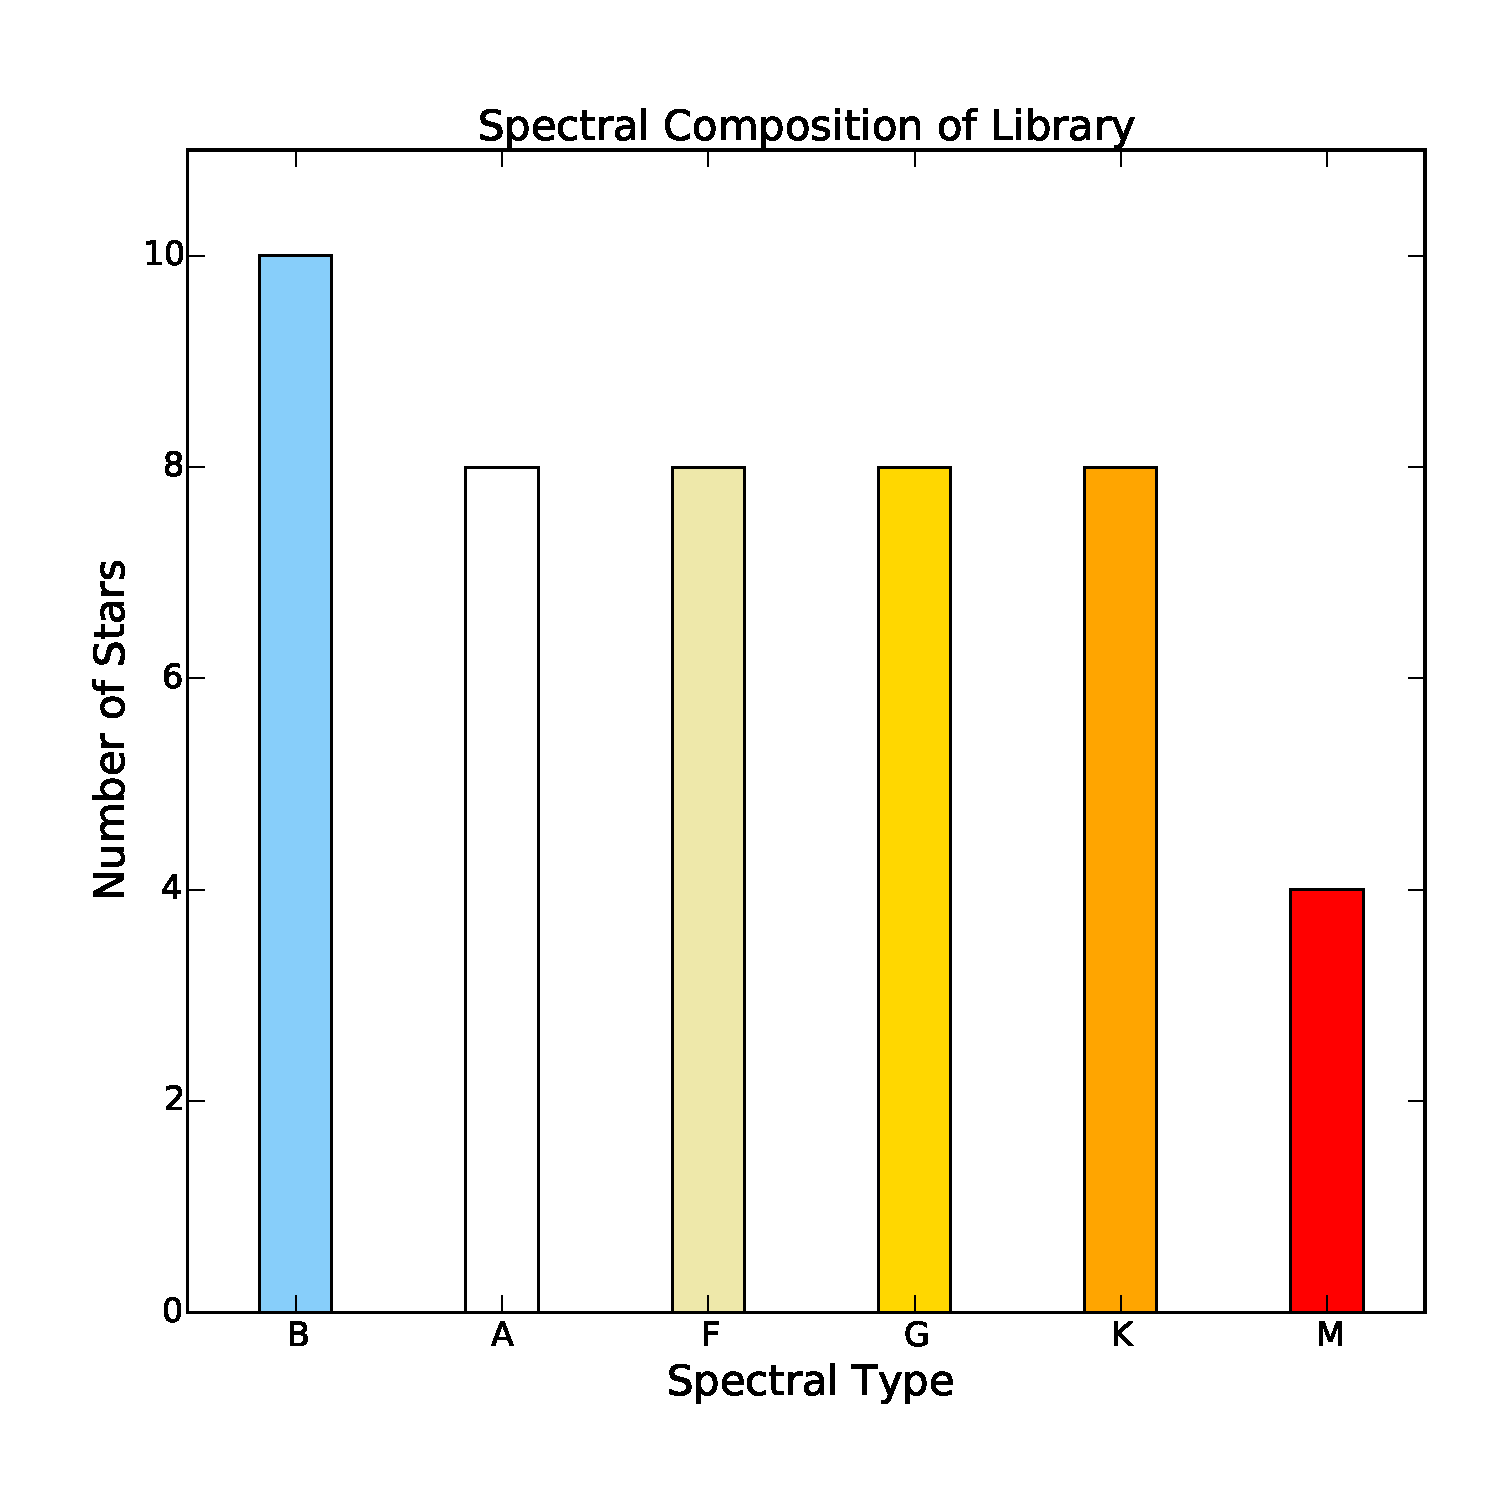
\includegraphics[height = 350px,width = 250px]{/Users/cmutnik/work/git/Spex-Young-Star-Atlas/figures/histogram_of_classes/spectral_color/histogram_color_46total}
\caption{ \protect{\bf Comparison of Spex \& uSpex} Shown here is a comparison of GSC 6801-186 using Spex before and after it was updated.}
\end{center}
\end{figure}

\subsection{Observations}

All of the objects discussed in this paper were observed between 
March 2012 and June 2015 (Table~\ref{tab:maintab}), with the 
NASA Infra-Red Telescope Facility (IRTF) and the SpeX 
instrument~\cite{Rayner_1998}. We used the short-wavelength cross-dispersed 
mode (SXD) with $R ∼ 2000$ matched to $0.3x15"$ slit.  Spex was upgraded in August 2014\footnote{See \url{http://irtfweb.ifa.hawaii.edu/~spex/SpeX_manual_06mar15.pdf} for details.}. 
%For reduction purposes, the Spex pipeline was used\footnote{\url{http://irtfweb.ifa.hawaii.edu/~spex/SpeX_manual_06mar15.pdf}}.  
%This upgrade increased Spex's wavelength sampling rate, allowing for higher accuracy of collected data 
This upgrade increased the observable wavelength range, filled 
in the gap around 1.8$\mu$m, and increased Spex's wavelength 
sampling rate, allowing for higher accuracy of collected data.
A portion of the objects in this catalog were observed prior to this upgrade.  
For this reason, it is necessary to compare data taken with each version of Spex (Table~\ref{tab:maintab}), 
shown in Figure~\ref{fig:uSpex-Spex}.
%, as shown in Figure~\ref{fig:uSpex-Spex}.  See Table~\ref{tab:maintab} for comparison.



GSC 06801-00186 was observed on June 29, 
2012 UT, before Spex was upgraded, and again on June 15, 2015, after uSpex 
was implemented~\cite{Spextool_Manual_Cushing_2015}.  Spectra collected after 
the upgrade span a larger wavelength range, but both Spex and uSpex data sufficiently 
cover the wavelength range needed for our study.  Data collected with both versions 
follow the same procedure, discussed below.  Before the upgrade, the wavelength 
range spanned 0.80-2.4~$\mu$m.  Following August 2014, the wavelength range 
was expanded to span 0.70-2.55~$\mu$m.\\

%  During observations, we collected two distinct types of data.  One set before Spex was updated and another after.  
 

%[HOW DO I PROPERLY CITE WAVELENGTH RANGE IN TABEL]\cite{RAYER_SPEX_OBSERVING_MANUAL_or_Spextool_2015_manual}.\\


During observations, integration times were altered as to maximize the Signal to Noise ratio (SNR).  
Observations were made in AB pairs.  After the initial A frame is taken, the telescope offsets ("nods") and captures a B frame.  Both frames are of the the same science target, at a different position along the slit.  Since our objects were treated as point sources, this AB mode allowed for the subtraction of the B frame from the A frame, leaving both positive and negative spectrum along with sky residuals~\cite{Cushing_2004}. Subtraction of these pairs allows for the removal of dark currents and sky residuals.



After collecting data on a particular science object, 
flat and arc calibration frames were taken.  
In order to minimize the time between target observations and 
the collection of calibration frames, the telescope remained unmoved.  
Background noise was identified and removed using darks and flats.



Standard A0V stars also needed to be observed, for telluric line corrections.  Which A0V 
to observe was determined by location and airmass.  For our purposes, an ideal A0V would 
deviate from the science objects' airmass by no more than 0.15 and be located 
in the same region of the sky as the science object.  This ensured minimal 
atmospheric derivations between our science and A0V stars.
%The airmass difference between a target and corresponding A0 never exceed 0.15.  
%Airmass of each A0 star differed from that of the targets by no more than 0.15.


\begin{table*}
\resizebox{\columnwidth}{!}{%
\caption{Listed here are observed targets with corresponding information.~\label{tab:maintab}}
\begin{tabular}{c|c|c|c|c|c|c|c|c|c|c|c|c}
Object & RA & DEC & Lit. Spectral Type & UT Date & J & SNR & Total Exp. Time & A0 standard & Teff (K) & 2Mass designation & other name & IRTF star used in comparison \\
 &  &  &  &  & (mag) &  & (s) &  &  &  &  &  \\
HD 146266 & 16:16:23.32 & -25:03:49.1 & A1V & 7/18/2012 & 7.533 & 210 & 120.0 & HD 145127 & 9320* & 2MASS J16162295-2503466 & -- & -- \\
HD 143472 & 16:01:26.93 & -25:11:56.6 & A2V & 7/18/2012 & 7.074 & 158 & 120.0 & HD 145127 & 8810 & 2MASS J16012664-2511545 & -- & -- \\
HD 145468 & 16:11:52.96 & -22:32:42.1 & A3V & 6/29/2012 & 7.45 & 126 & 300.0 & HD 145188 & 8490* & 2MASS J16115266-2232421 & -- & -- \\
HD 142424 & 15:55:17.16 & -23:22:17.4 & A4V & 7/18/2012 & 7.54 & 138 & 180.0 & HD 144254 & 8230* & 2MASS J15551758-2322036 & -- & -- \\
HD 142097 & 15:53:21.87 & -21:58:20.6 & A5V & 7/12/2012 & 7.493 & 129 & 120.0 & HD 145188 & 8160 & 2MASS J15532192-2158165 & -- & -- \\
HD 146899 & 16:19:38.05 & -26:52:31.6 & A8V & 6/29/2012 & 8.569 & 206 & 540.0 & HD 146606 & 7610* & 2MASS J16193785-2652308 & -- & -- \\
HIP 73990 & 15:07:14.53 & -29:30:01.5 & A9V & 6/15/2015 & 7.499 & 130 & 88.9632 & HD 141091 & 7470* & 2MASS J15071494-2930160 & HD 133803 & -- \\
HD 147137 & 16:20:50.48 & -22:35:45.2 & A9V & 7/12/2012 & 8.032 & 146 & 600.0 & HD 145127 & 7470* & 2MASS J16205022-2235387 & -- & -- \\
HIP 78933 & 16:06:48.64 & -20:40:02.7 & B1V & 6/15/2015 & 4.16 & 126 & 27.801 & HD 138813 & 25600 & 2MASS J16064842-2040088 & * ome Sco & -- \\
HD 144470 & 16:06:48.96 & -20:40:14.4 & B1V & 7/12/2012 & 4.16 & 44 & 60.0 & HD 138813 & 25600 & 2MASS J16064842-2040088 & * ome Sco & -- \\
HD 138485 & 15:32:55.67 & -16:51:16.5 & B3V & 7/12/2012 & 5.78 & 129 & 200.0 & HD 133466 & 19000 & 2MASS J15325521-1651101 & * zet04 Lib & -- \\
HD 147196 & 16:21:19.54 & -23:42:34.9 & B6/B7Vn & 7/12/2012 & 6.565 & 16 & 600.0 & HD 138813 & 14100 & 2MASS J16211918-2342287 & -- & -- \\
HIP 70753 & 14:28:10.35 & -29:29:26.1 & B8V & 6/15/2015 & 5.073 & 149 & 27.801 & HD 112305 & 11800 & 2MASS J14281043-2929299 & * I Hya & -- \\
HIP 77909 & 15:54:38.54 & -25:14:42.4 & B8V & 6/15/2015 & 5.925 & 125 & 27.801 & HD 138813 & 11800 & 2MASS J15543952-2514375 & * 3 Sco & -- \\
HIP 79031 & 16:07:51.15 & -24:27:47.7 & B8V & 6/15/2015 & 6.379 & 129 & 27.801 & HD 133750 & 11800 & 2MASS J16075188-2427443 & HR 5998 & -- \\
HIP 78207 & 15:58:11.48 & -14:16:40.6 & B8V & 6/15/2015 & 5.098 & 144 & 27.801 & HD 125299 & 11800 & 2MASS J15581136-1416454 & * 48 Lib & -- \\
HD 144661 & 16:07:51.99 & -24:27:42.8 & B8V & 7/18/2012 & 6.379 & 117 & 90.0 & HD 143715 & 11800 & 2MASS J16075188-2427443 & HR 5998 & -- \\
HIP 76633 & 15:39:00:11 & -19:43:50.9 & B9V & 6/15/2015 & 7.476 & 101 & 58.3824 & HD 125299 & 10700 & 2MASS J15390006-1943569 & HD 139486 & -- \\
HIP 79599 & 16:14:28.97 & -21:06:20.4 & B9V & 6/15/2015 & 6.342 & 121 & 58.3824 & HD 145188 & 10700 & 2MASS J16142888-2106274 & HR 6051 & -- \\
HD 143567 & 16:01:55.60 & -21:58:50.4 & B9V & 7/18/2012 & 6.928 & 119 & 120.0 & HD 145188 & 10700 & 2MASS J16015546-2158496 & -- & -- \\
HD 137130 & 15:25:08.91 & -26:34:30.9 & F0V & 3/22/2012 & 7.566 & 160 & 1200.0 & HD 146236 & 7020/7320* & 2MASS J15250939-2634310 & -- & -- \\
HIP 79369 & 16:11:55.19 & -21:06:10.4 & F1V & 6/15/2015 & 7.855 & 101 & 177.926 & HD 145188 & 7160* & 2MASS J16115551-2106179 & HD 145467 & -- \\
HIP 82319 & 16:49:10.74 & -22:42:46.5 & F3V & 6/15/2015 & 8.05 & 117 & 597.722 & HD 159008 & 6810* & 2MASS J16491221-2242416 & HD 151594 & -- \\
HD 146743 & 16:18:39.41 & -21:35:39.6 & F3V & 7/12/2012 & 7.838 & 191 & 360.0 & HD 145188 & 6810* & 2MASS J16183914-2135341 & -- & -- \\
HD 148153 & 16:27:12.68 & -27:11:27.2 & F5V & 7/12/2012 & 7.419 & 133 & 300.0 & HD 145188 & 6530 & 2MASS J16271252-2711219 & -- & -- \\
HIP 78977 & 16:07:17.56 & -22:03:39.8 & F7V & 6/29/2012 & 7.543 & 204 & 240.0 & HD 144254 & 6240 & 2MASS J16071778-2203364 & -- & -- \\
HIP 71982 & 14:43:19.42 & -10:35:13.5 & F8V & 6/15/2015 & 7.474 & 130 & 88.9632 & HD 124683 & 6250 & 2MASS J14431929-1035194 & HD 129520 & -- \\
HD 142113 & 15:53:21.17 & -19:23:58.8 & F8V & 7/12/2012 & 7.782 & 176 & 240.0 & HD 143715 & 6250 & 2MASS J15532089-1923535 & -- & -- \\
HIP 61412 & 12:35:00.73 & -26:42:46.3 & G0V & 6/15/2015 & 7.162 & 127 & 27.801 & HD 114345 & 5930 & 2MASS J12350095-2642454 & HD 109454 & -- \\
HD 148040 & 16:26:29.32 & -27:41:17.0 & G0V & 3/22/2012 & 7.554 & 234 & 720.0 & HD 141091 & 5930 & 2MASS J16262991-2741203 & -- & -- \\
HD 133748 & 15:06:51.76 & -23:37:27.6 & G2V & 3/22/2012 & 8.251 & 164 & 1200.0 & HD 138813 & 5830 & 2MASS J15065202-2337277 & -- & -- \\
GSC 06793-00994 & 16:14:02.15 & -23:01:08.0 & G4V & 7/12/2012 & 9.375 & 131 & 600.0 & HD 141091 & 5740 & 2MASS J16140211-2301021 & -- & -- \\
HBC 649 & 16:34:09.09 & -15:48:01.4 & G5V & 6/15/2015 & 8.995 & 137 & 478.18 & HD 159008 & 5560 & 2MASS J16340916-1548168 & V* V1003 Oph & -- \\
GSC 06801-00186 (oldSpx) & 16:14:59.03 & -27:50:27.1 & K0IV(e) & 6/29/2012 & 9.334 & 136 & 240.0 & HD 146606 & -- & 2MASS J16145918-2750230 & -- & -- \\
GSC 06801-00186 & 16:14:59:30 & -27:50:17.9 & K0IV(e) & 6/15/2015 & 9.334 & 105 & 447.597 & HD 146606 & -- & 2MASS J16145918-2750230 & -- & -- \\
GSC 06793-01406 & 16:16:17.80 & -23:39:51.3 & G7V & 6/29/2012 & 8.727 & 151 & 240.0 & HD 145127 & 5500* & 2MASS J16161795-2339476 & -- & -- \\
GSC 06213-00306AB & 16:13:18.19 & -22:12:52.3 & G9V & 6/29/2012 & 8.18 & 143 & 90.0 & HD 145188 & 5270* & 2MASS J16131858-2212489 & -- & -- \\
CD-25 11942 & 17:06:00.85 & -25:20:25.9 & K0V & 6/15/2015 & 8.099 & 160 & 297.471 & HD 170364 & 5240 & 2MASS J17060119-2520302 & -- & -- \\
ScoPMS 214 & 16:29:48.69 & -21:52:17.2 & K0 / K2IV(e) & 7/12/2012 & 8.677 & 190 & 270.0 & HD 145188 & 5240/ & 2MASS J16294869-2152118 & V* V2505 Oph & -- \\
HD 141813 & 15:51:54.35 & -26:22:09.2 & K0 / K1III+ & 7/12/2012 & 8.232 & 30 & 180.0 & HD 146606 & 5240/4610 & 2MASS J15515438-2622054 & -- & -- \\
HD 14311 & 15:58:57.31 & -13:10:14.3 & K0III & 7/12/2012 & 7.263 & 62 & 40.0 & HD 133466 & 4810 & 2MASS J02205232+5853189 & -- & -- \\
ScoPMS 44 & 16:11:08.86 & -19:04:51.8 & K2 / K2IV(e) & 7/12/2012 & 8.761 & 136 & 180.0 & HD 144925 & 5010 & 2MASS J16110890-1904468 & Wa Oph 1 & -- \\
GSC 06793-00797 & 16:13:02.68 & -22:57:49.2 & K4V & 6/29/2012 & 9.322 & 127 & 270.0 & HD 142705 & 4560 & 2MASS J16130271-2257446 & -- & -- \\
ScoPMS 45 & 16:11:20.40 & -18:20:59.6 & K5V & 7/12/2012 & 9.492 & 152 & 600.0 & HD 144254 & 4340 & 2MASS J16112057-1820549 & V* V1157 Sco & -- \\
GSC 06208-00834 & 16:06:31.65 & -20:36:26.6 & K6V & 6/29/2012 & 9.731 & 120 & 540.0 & HD 144254 & 4300* & 2MASS J16063169-2036232 & -- & -- \\
Sco 160900.7-19085 & 16:09:00.79 & -19:08:56.0 & K9V & 6/29/2012 & 10.22 & 159 & 600.0 & HD 144925 & 3910* & 2MASS J16090075-1908526 & -- & -- \\
GSC 06213-00194 & 16:13:18.65 & -22:12:53.6 & M0V & 6/29/2012 & 9.483 & 179 & 120.0 & HD 145188 & 3800 & 2MASS J16094098-2217594 & -- & -- \\
RX J1602.0-2221 & 16:02:00.39 & -22:21:23.7 & M1V & 6/29/2012 & 9.824 & 116 & 600.0 & HD 138813 & 3680 & 2MASS J16020039-2221237 & -- & -- \\
ScoPMS 008b & 15:55:16.86 & -23:22:29.8 & M2.5V & 7/18/2012 & 10.294 & 96 & 900.0 & HD 143715 & 3440* & 2MASS J15551704-2322165 & -- & -- \\
ScoPMS 46 & 16:11:29.93 & -18:50:56.2 & M4V & 7/18/2012 & 10.751 & 114 & 540.0 & HD 144254 & 3180 & 2MASS J16112979-1850541 & -- & -- \\
HIP 78721 & 16:04:14.14 & 50:30:03.7 & SC5.5-C71e & 7/12/2012 & 5.204 & 21 & 240.0 & HD 133466 & -- & 2MASS J16041342+5029567 & V* RR Her & -- \\
RX J1558.2-2328 & 15:58:12.83 & -23:28:41.9 & G9V & 7/12/2012 & 8.574 & 199 & 360.0 & HD 145127 & 5270* & 2MASS J15581270-2328364 & -- & -- \\
\end{tabular}
}
\end{table*}

%\begin{table}
%\begin{center}
%\caption{Listed here are observed targets with corresponding information.~\label{tab:maintab}}
%\begin{tabular}{c|c|c|c|c|c|c|c|c|c|c|c|c}

Effective temperatures with no identifying symbol come from from~\cite{Astrophysical_Quantities_Ed4}.  
A least-squares fit to published values allowed for determination of 
temperatures for unlisted spectral types.  Only values pertaining to specific 
luminosity classes were used in each fit.



%\end{tabular}
%\caption{
%	{\bf Notes.}~$^{*}$ Indicates temperatures determined by interpolation; with values rounded to tens place.\\
%	{\bf References.} (1); (2)...
%}
%\end{center}
%\end{table}
\subsection{Data Reduction}

%[ORDERING: aov for telluric...the choice of ao is standard...the obs a0 was comp vega]
For reduction of collected spectra, Spextool was used~\cite{Cushing_2004}. 
Calibration frames consist of flats, arcs, and A0V standards.  Flat frames allow for the removal of inconsistencies, amongst the detector's pixels.  Observations of an arc lamp permitted wavelength calibration.  The choice of A0V stars as standards was based on their relatively few spectral features, outside hydrogen lines; making isolation of telluric lines significantly cleaner.  
For telluric reduction, an observed A0V star was compared to Vega.  Deviations of the observed star, from the standard, are attributed to atmospheric interference.  The same atmospheric disturbances apply to all objects observed at the same time and airmass.  Telluric corrections were accomplished using spectroscopic observations of standard stars. B--V data, provided by Simbad~\cite{simbad}, was used in in the standard selection process.
In order to properly scale emission lines and account for velocity shifts, a kernel was constructed using the observed A0V.  Finally, all orders were scaled and merged, producing a continuous spectrum.
A more detailed account of this process is outlined by Vacca~\cite{Vacca_2003}.  
%This process allows for such telluric residuals to be removed.  
%Telluric corrections can now be applied to the spectra of each science object.~\cite{Cushing_2004}



To be transformed from an array into a workable spectrum Spextool~\cite{Cushing_2004} was used.  Once extracted, each spectra was visually reviewed.  Hot pixels, outliers, and areas of low SNR were masked and removed.  Through this process, the intrinsic spectrum of each star was better revealed.  SNR calculations occurred between 2.025--2.162~$\mu$m.  
%All stars in this sample have SNR between 95 -- 240.
All stars in this sample have SNR above 95.

\begin{figure}[h!]
\begin{center}
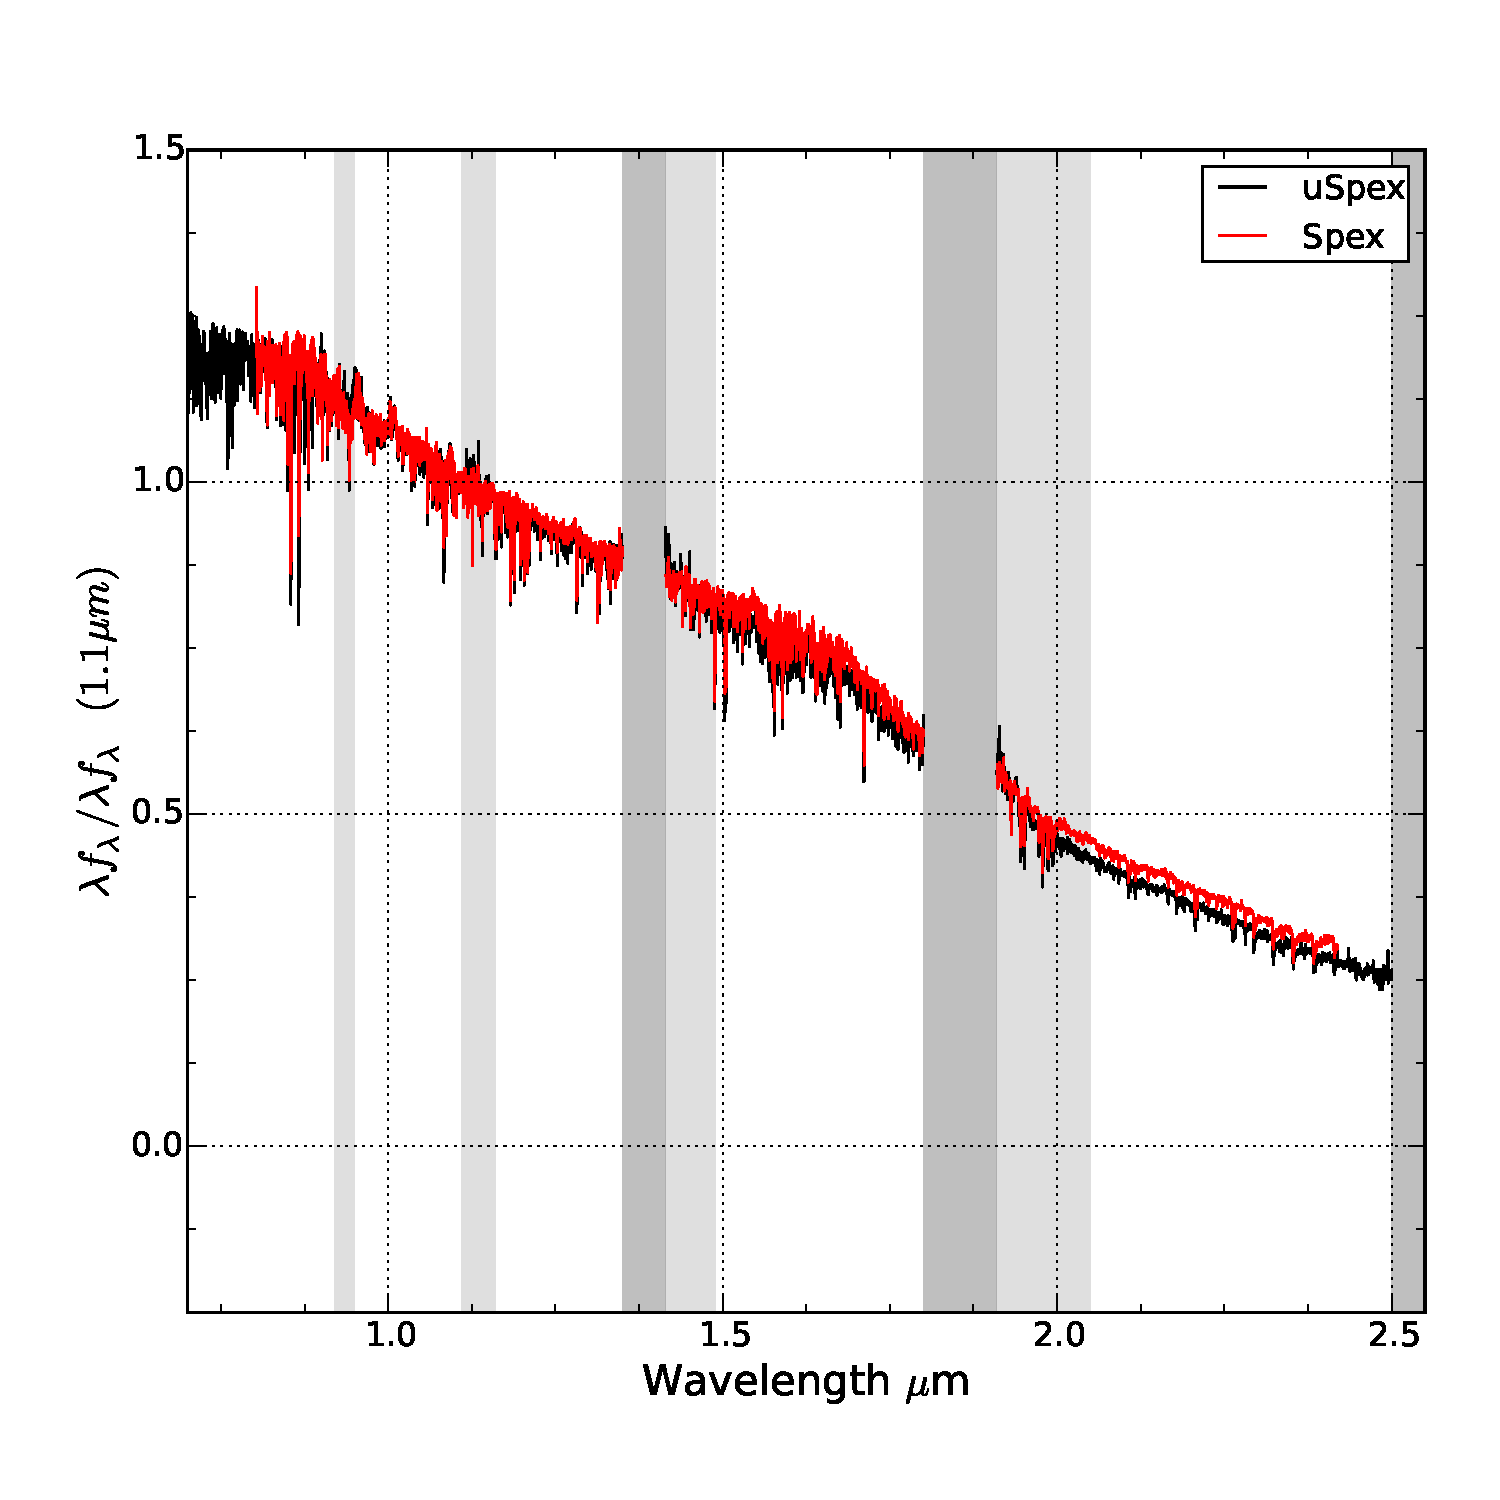
\includegraphics[height = 350px,width = 250px]{/Users/cmutnik/work/git/Spex-Young-Star-Atlas/figures/spex_uspex/single_stacked_mask_tics}
\caption{ \protect{\bf Comparison of Spex \& uSpex} Shown here is a comparison of GSC 6801-186 using Spex before and after it was updated.}
\end{center}
\end{figure}

\section{Data and Analysis}

%Comparison of the data taken on each A0V standard to that of a well known A0V, Vega, allowed for the determination of atmospheric residuals.  %Spextool made this data reduction possible.  
%For reduction purposes, the Spex pipeline was used\footnote{\url{http://irtfweb.ifa.hawaii.edu/~spex/SpeX_manual_06mar15.pdf}}.  The difference between an observed A0V and the model for Vega can be attributed to atmospheric conditions existing at the time of observation.  

\subsection{The Spectra}

\iffalse
	{\bf List of stars with multiple spectral type references in literature with notes:}\\
	\begin{itemize}
		\item{} CD-25 11942
		\item{}~~~match isn't great

		\item{} GSC 06213-00306AB
		\item{}~~~missing exact match in comparison plot

		\item{} GSC 06793-00797
		\item{}~~~match isn't great

		\item{} GSC 06793-01406
		\item{}~~~missing exact match in comparison plot

		\item{} GSC 06801-00186
		\item{}~~~missing exact match in comparison plot

		\item{} HIP 78977
		\item{}~~~could be F7 or F8

		\item{} HIP 79369
		\item{}~~~could be F1 or F0

		\item{} ScoPMS 44
		\item{}~~~match isn't great

		\item{} ScoPMS 214
		\item{}~~~match isn't great
	\end{itemize}
\fi

[See commented-out list above]\\


Of the 46 stars composing this atlas, 9 have more than one spectral type 
referenced in the literature.   For such stars, spectral classes referenced 
in Table~\ref{tab:maintab} were determined by visual examination of individual 
spectra.  Observed spectra were compared to existing libraries, with established 
spectral classes.  References were chosen based on EW values and comparison of 
spectral features.\\


\noindent [{\bf section 3.1 Rayner}]\\
\noindent [Digital copies of the spectra, with associated information, can be found at $----$.]\\
\noindent [Each spectra is available as a fits or png file.]\\
\noindent [Discuss masking of telluric regions.]\\





\begin{figure}[h!]
\begin{center}
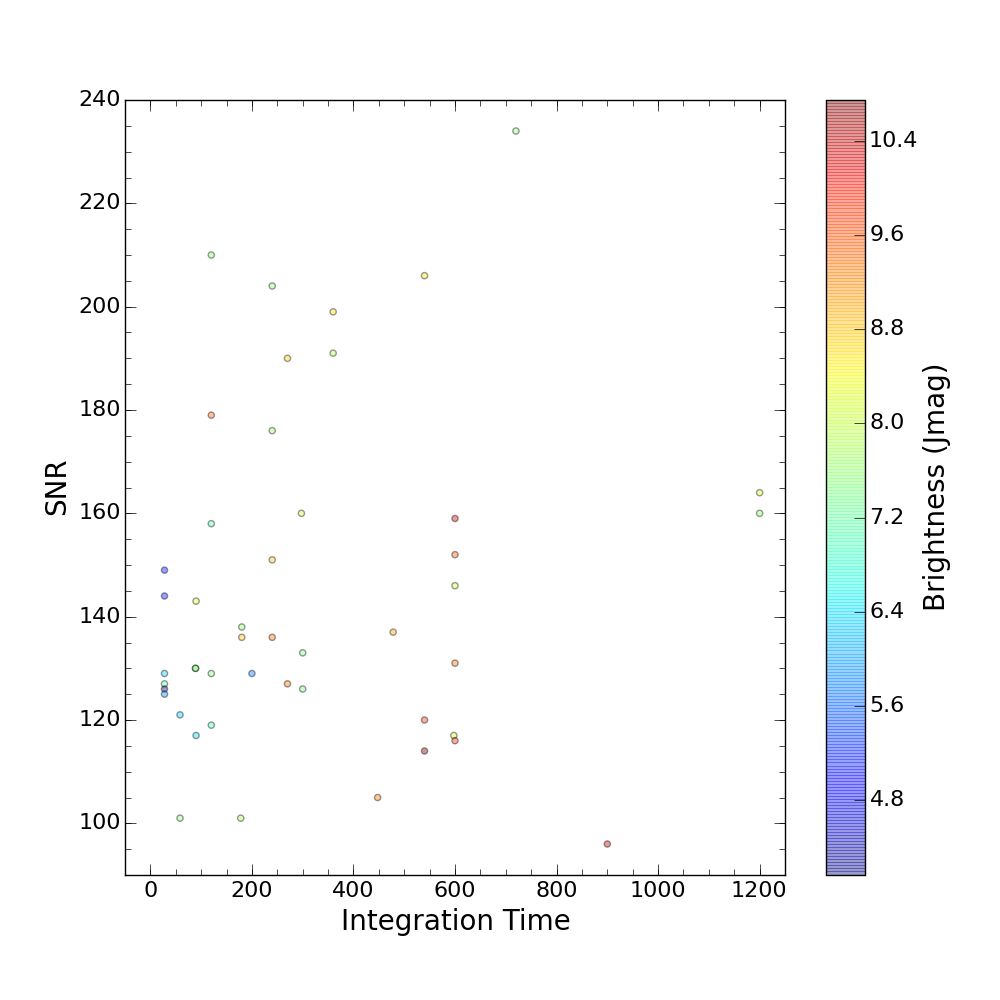
\includegraphics[height = 350px,width = 250px]{/Users/cmutnik/work/git/Spex-Young-Star-Atlas/figures/SNR_brightness/snr_exptime}
\caption{ \protect{\bf Comparison of Spex \& uSpex} Shown here is a comparison of GSC 6801-186 using Spex before and after it was updated.}
\end{center}
\end{figure}


\begin{figure}[h!]
\begin{center}
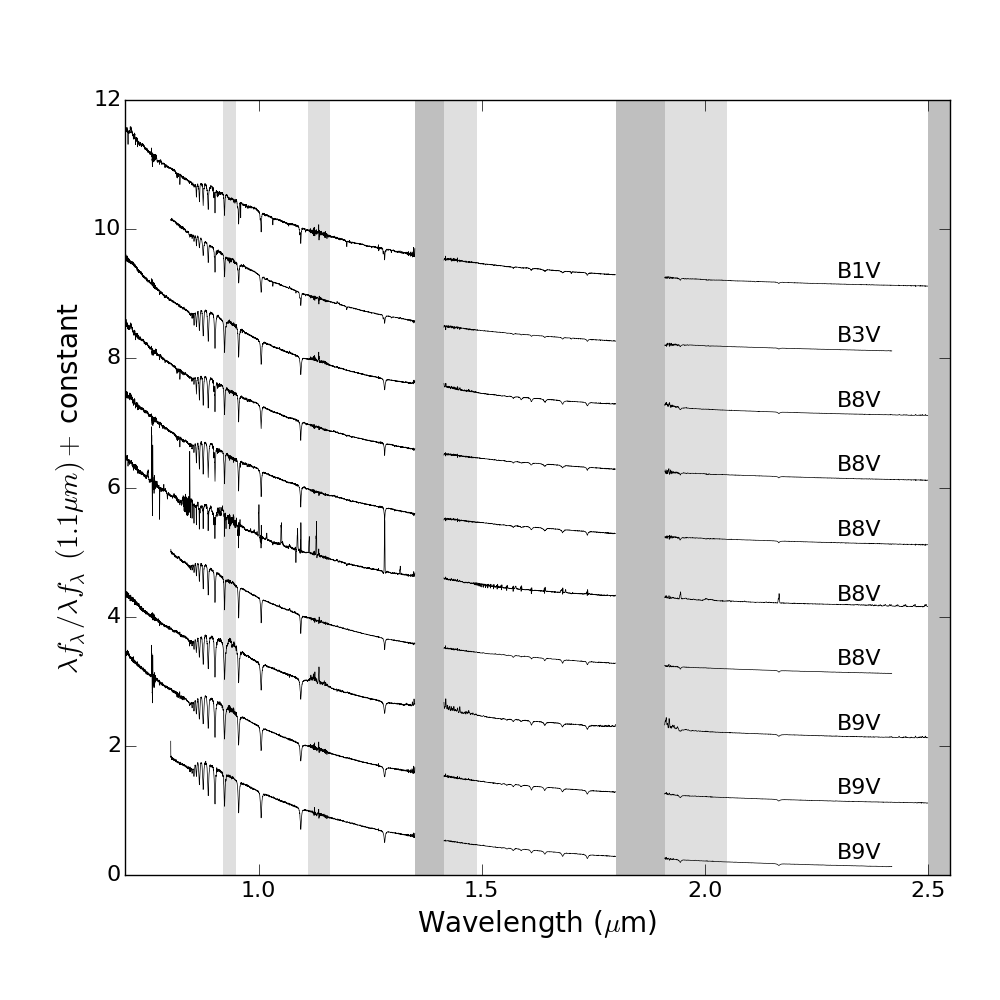
\includegraphics[height = 350px,width = 250px]{/Users/cmutnik/work/git/Spex-Young-Star-Atlas/figures/stacked_plots/b/group_b.png}
\caption{ \protect{\bf Comparison of Spex \& uSpex} Shown here is a comparison of GSC 6801-186 using Spex before and after it was updated.}
\end{center}
\end{figure}


\begin{figure}[h!]
\begin{center}
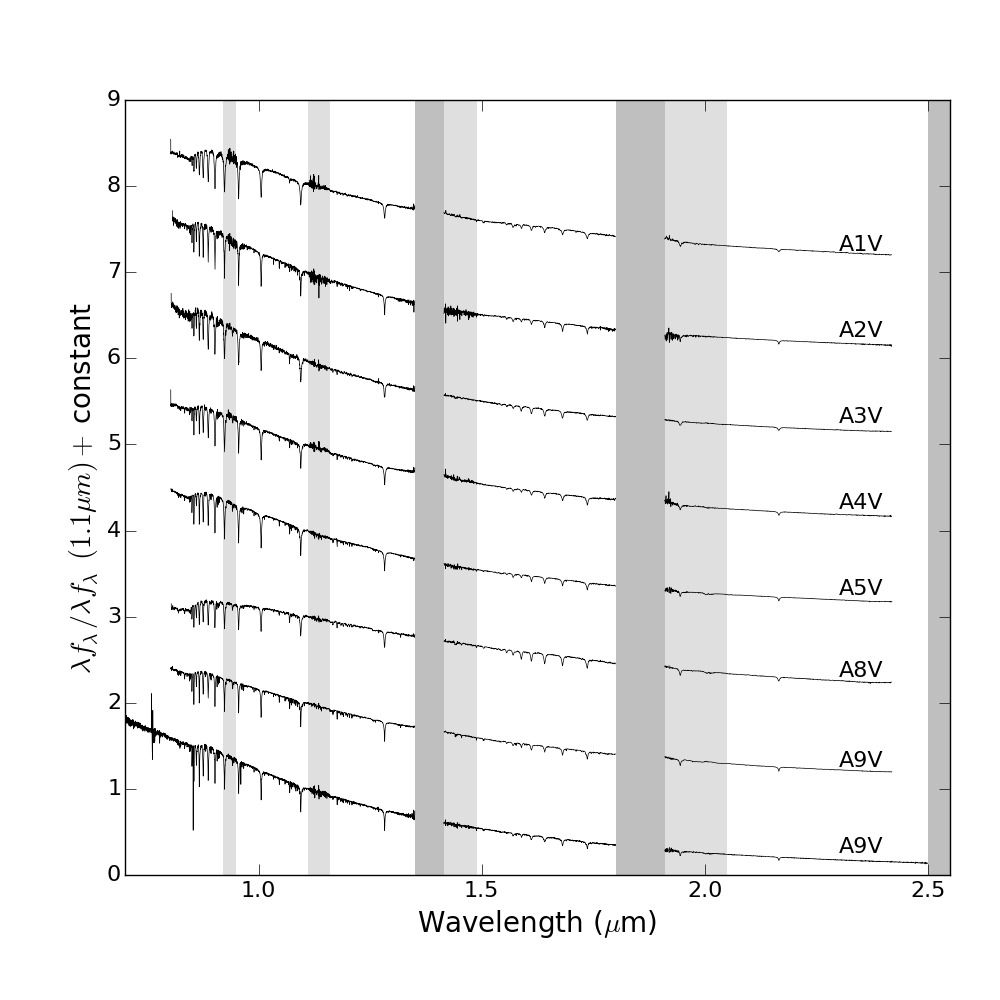
\includegraphics[height = 350px,width = 250px]{/Users/cmutnik/work/git/Spex-Young-Star-Atlas/figures/stacked_plots/a/group_a.png}
\caption{ \protect{\bf Comparison of Spex \& uSpex} Shown here is a comparison of GSC 6801-186 using Spex before and after it was updated.}
\end{center}
\end{figure}


\begin{figure}[h!]
\begin{center}
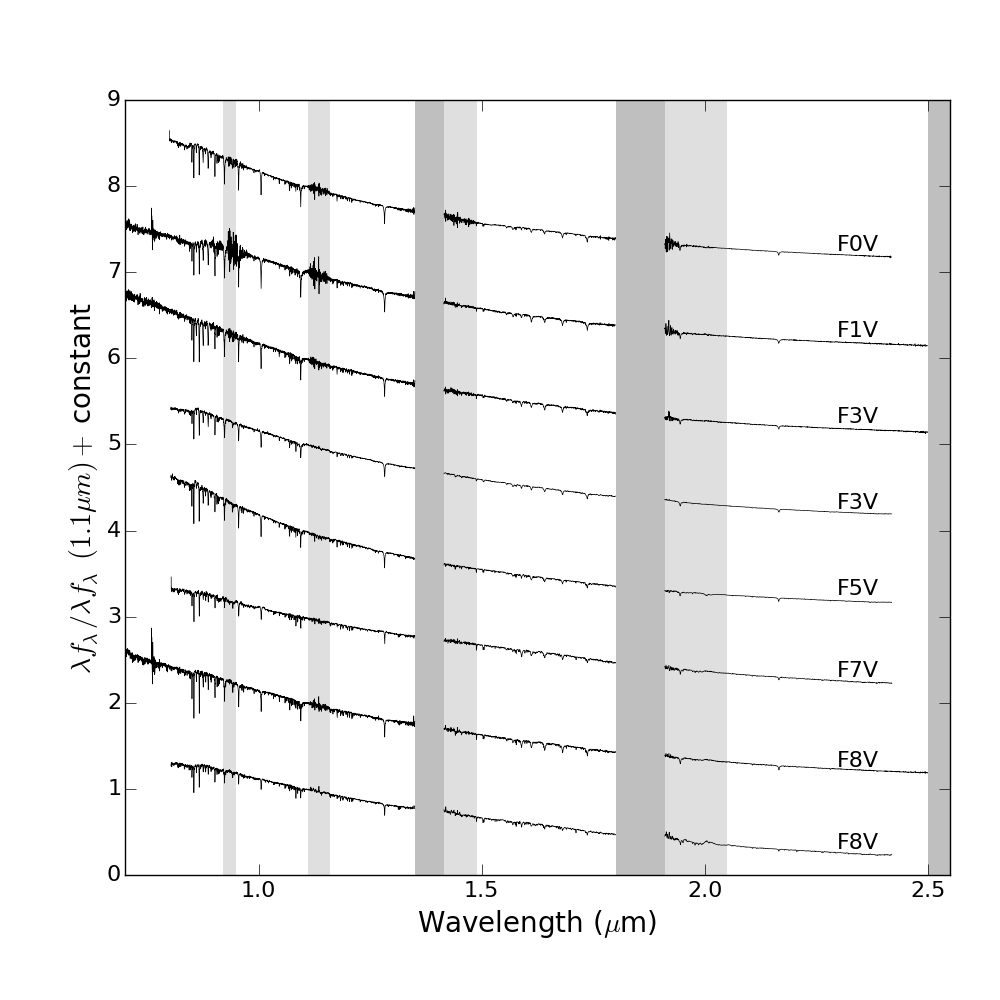
\includegraphics[height = 350px,width = 250px]{/Users/cmutnik/work/git/Spex-Young-Star-Atlas/figures/stacked_plots/f/group_f.png}
\caption{ \protect{\bf Comparison of Spex \& uSpex} Shown here is a comparison of GSC 6801-186 using Spex before and after it was updated.}
\end{center}
\end{figure}


\begin{figure}[h!]
\begin{center}
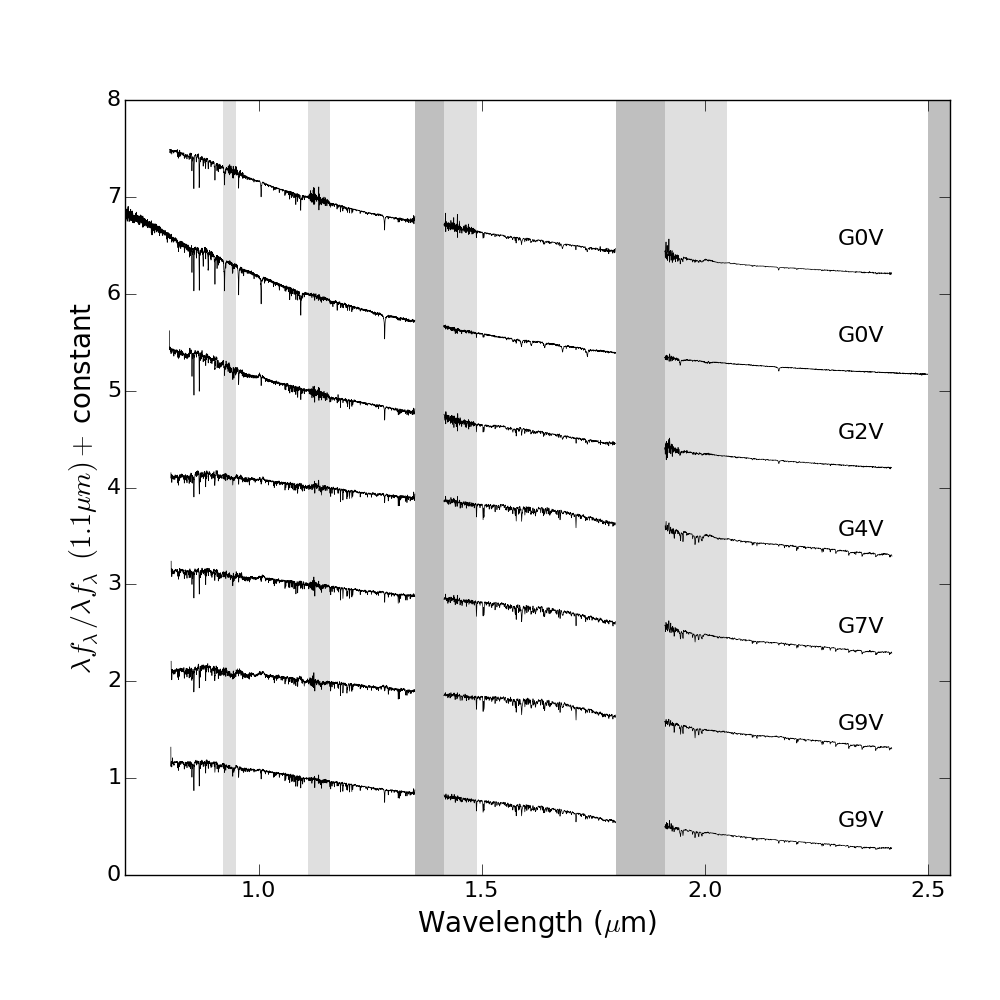
\includegraphics[height = 350px,width = 250px]{/Users/cmutnik/work/git/Spex-Young-Star-Atlas/figures/stacked_plots/g/group_g.png}
\caption{ \protect{\bf Comparison of Spex \& uSpex} Shown here is a comparison of GSC 6801-186 using Spex before and after it was updated.}
\end{center}
\end{figure}


\begin{figure}[h!]
\begin{center}
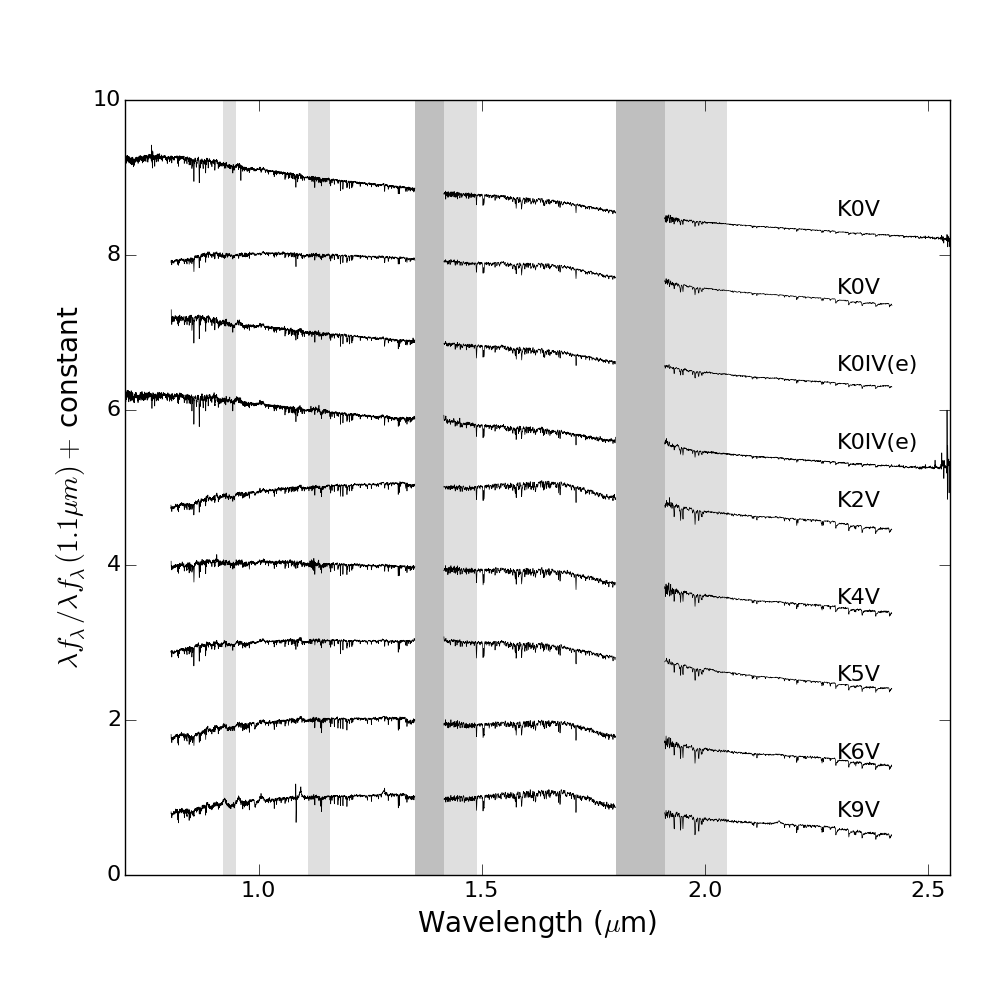
\includegraphics[height = 350px,width = 250px]{/Users/cmutnik/work/git/Spex-Young-Star-Atlas/figures/stacked_plots/k/group_k.png}
\caption{ \protect{\bf Comparison of Spex \& uSpex} Shown here is a comparison of GSC 6801-186 using Spex before and after it was updated.}
\end{center}
\end{figure}


\begin{figure}[h!]
\begin{center}
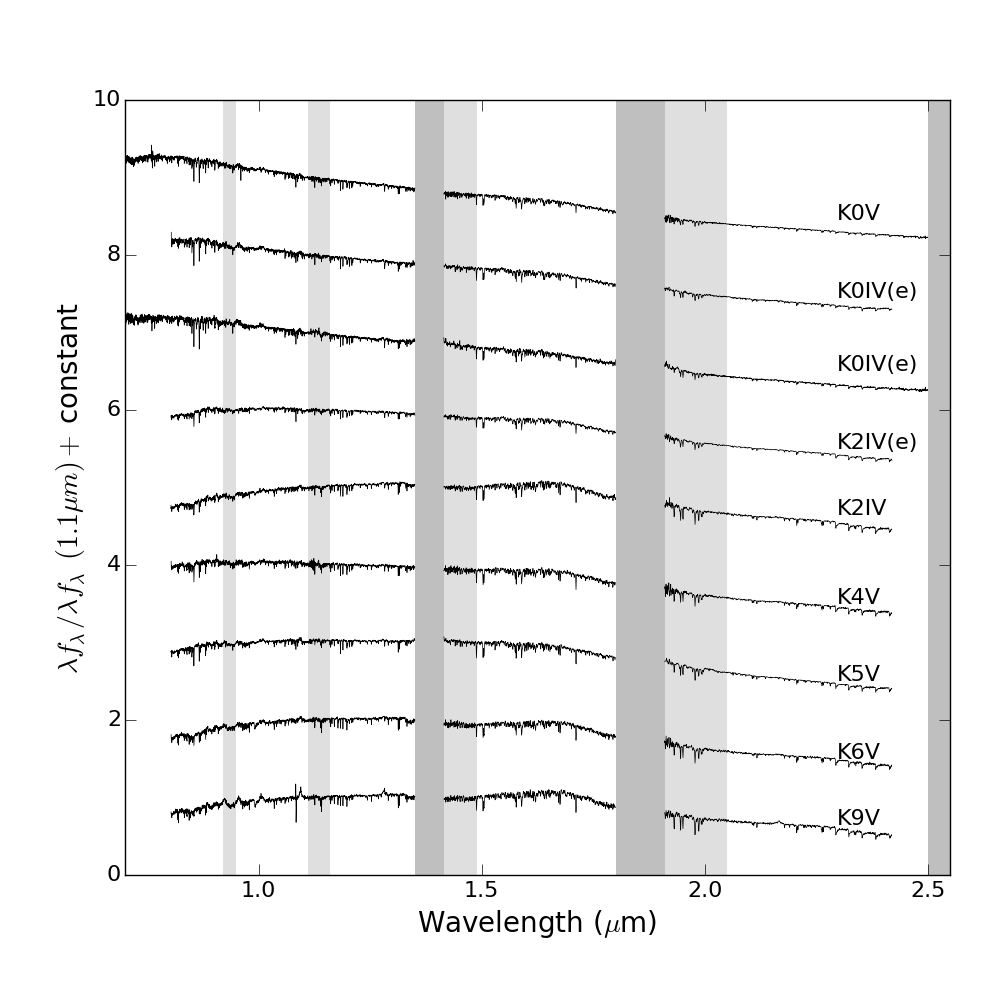
\includegraphics[height = 350px,width = 250px]{/Users/cmutnik/work/git/Spex-Young-Star-Atlas/figures/stacked_plots/other/k_doubleCount/group_k_doubleCount.png}
\caption{ \protect{\bf Comparison of Spex \& uSpex} Shown here is a comparison of GSC 6801-186 using Spex before and after it was updated.}
\end{center}
\end{figure}


\begin{figure}[h!]
\begin{center}
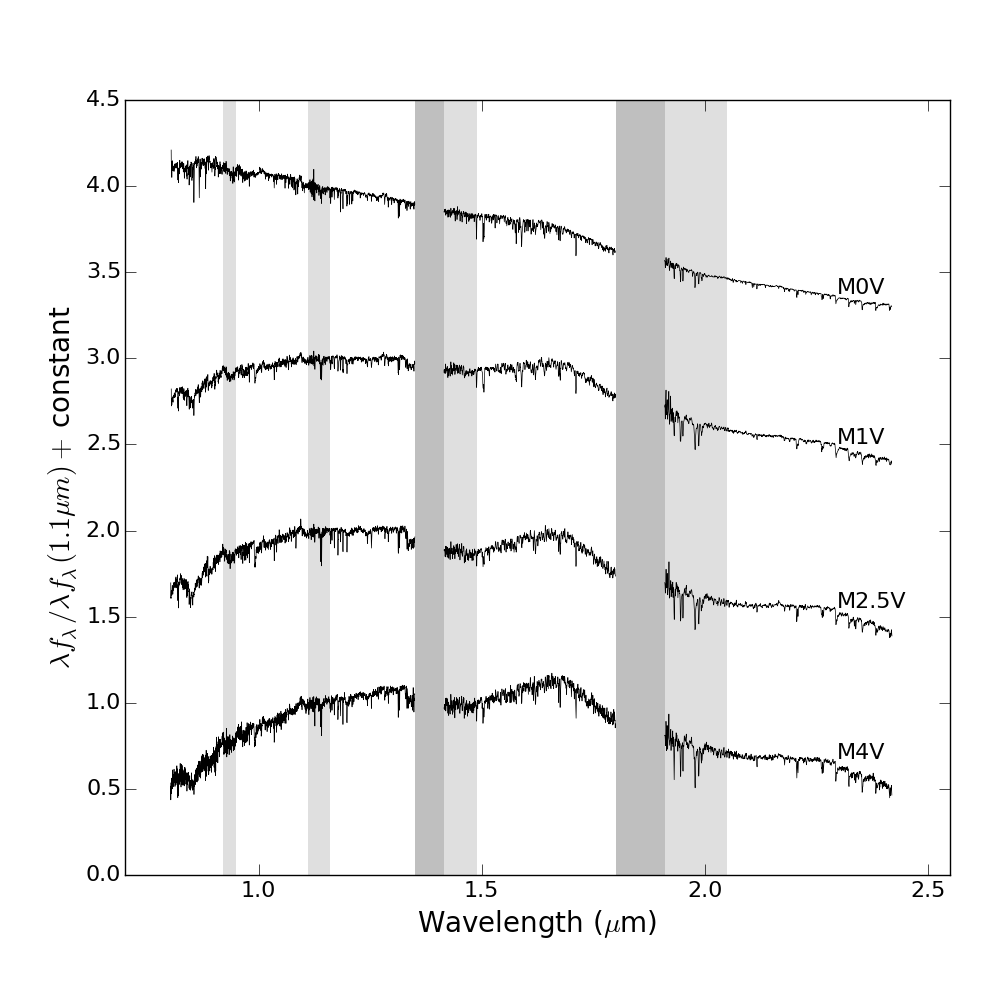
\includegraphics[height = 350px,width = 250px]{/Users/cmutnik/work/git/Spex-Young-Star-Atlas/figures/stacked_plots/m/group_m.png}
\caption{ \protect{\bf Comparison of Spex \& uSpex} Shown here is a comparison of GSC 6801-186 using Spex before and after it was updated.}
\end{center}
\end{figure}


\begin{figure}[h!]
\begin{center}
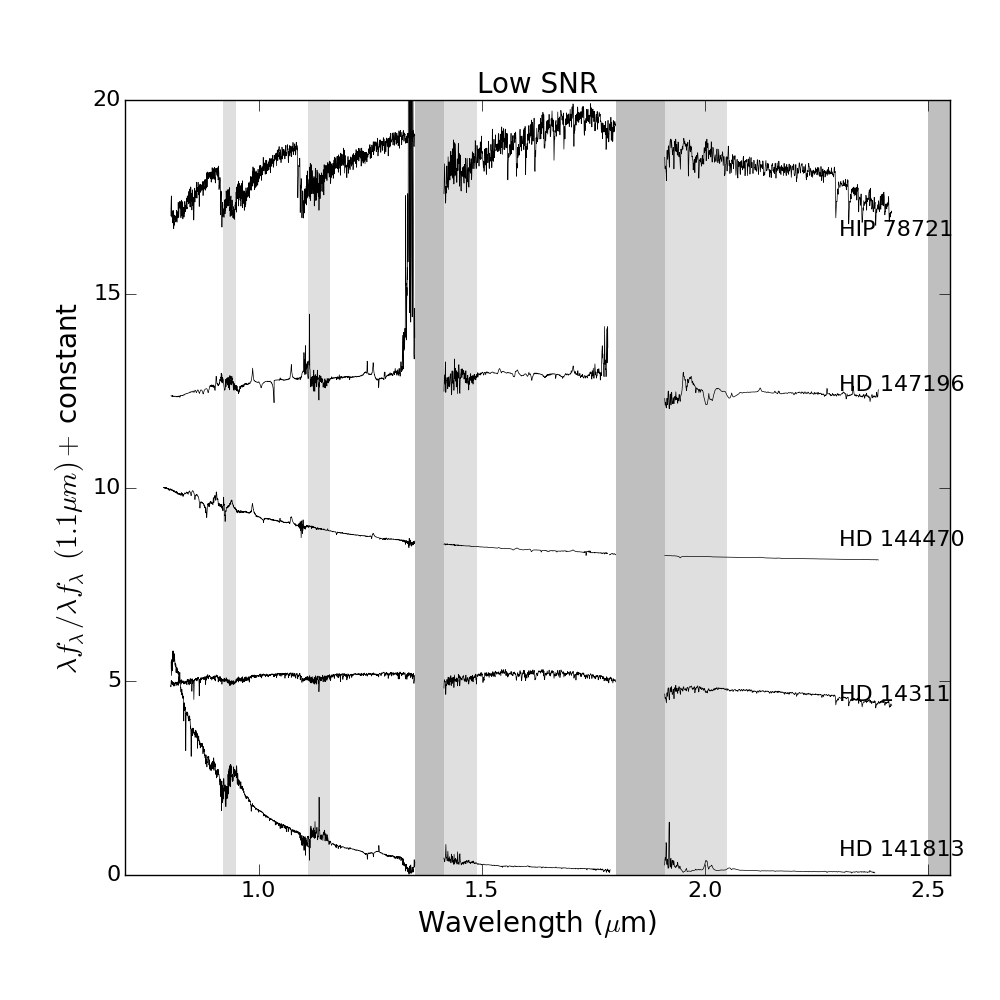
\includegraphics[height = 350px,width = 250px]{/Users/cmutnik/work/git/Spex-Young-Star-Atlas/figures/stacked_plots/other/low_snr/group_low_SNR.png}
\caption{ \protect{\bf Comparison of Spex \& uSpex} Shown here is a comparison of GSC 6801-186 using Spex before and after it was updated.}
\end{center}
\end{figure}


\begin{figure}[h!]
\begin{center}
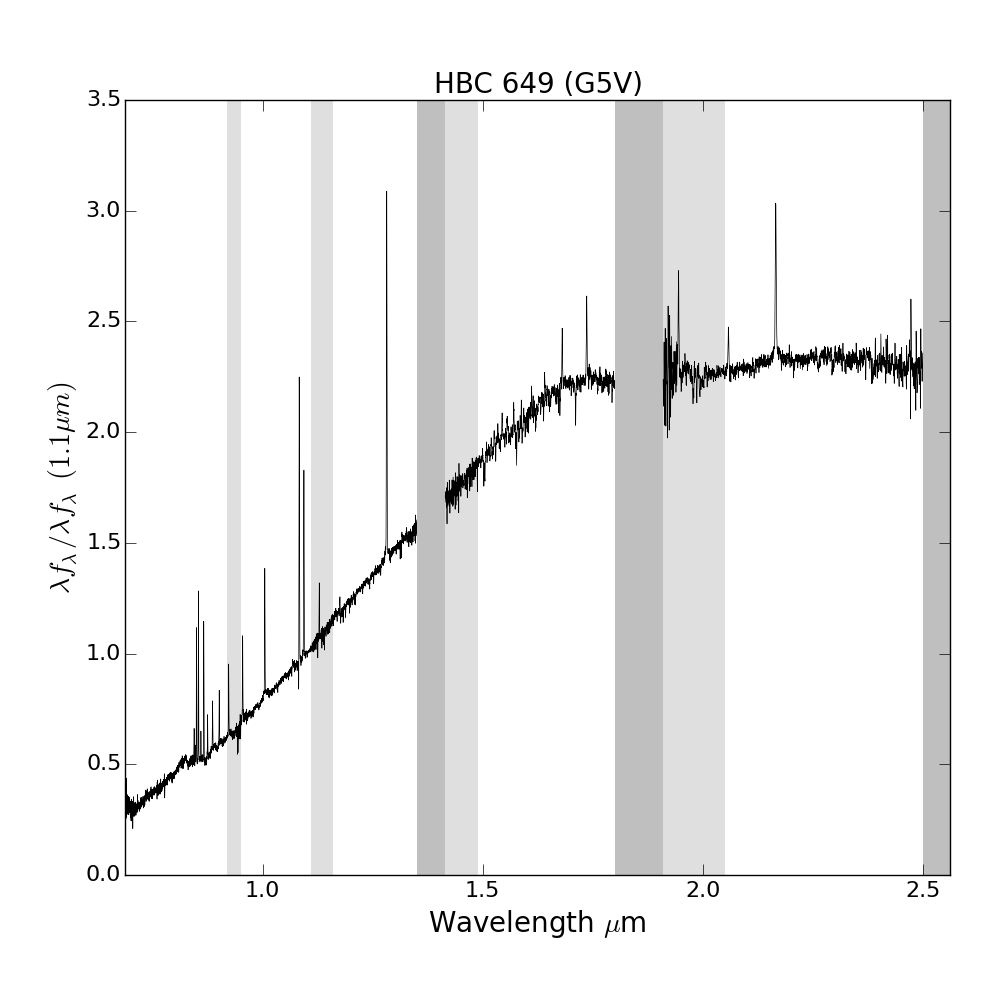
\includegraphics[height = 350px,width = 250px]{/Users/cmutnik/work/git/Spex-Young-Star-Atlas/figures/stacked_plots/other/g5v/g5v_HBC_649}
\caption{ \protect{\bf Comparison of Spex \& uSpex} Shown here is a comparison of GSC 6801-186 using Spex before and after it was updated.}
\end{center}
\end{figure}

\begin{table}[H]
    \caption{EW Limit Definitions\tablefootnote{Table 8 of~\cite{Rayner_2009}.}.~\label{tab:features}}
	\begin{tabular}{l c c c}
		Feature & Feature Limits ($\mu$m) & First Continuum Level Limits ($\mu$m) & Second Continuum Level Limits ($\mu$m) \\ \hline
		Ca II (0.866~$\mu$m) & 0.8655--0.8673 & 0.862--0.864 & 0.870--0.873 \\
		Na I (1.14~$\mu$m) & 1.137--1.1428 & 1.125--1.130 & 1.150--1.160 \\
		Al I (1.313~$\mu$m) & 1.3118--1.3165 & 1.305--1.309 & 1.320--1.325 \\
		Mg I (1.485~$\mu$m) & 1.4867--1.4895 & 1.4775--1.485 & 1.491--1.497 \\
		Mg I (1.711~$\mu$m) & 1.7098--1.7130 & 1.702--1.708 & 1.715--1.720 \\
		Na I (2.206~$\mu$m) & 2.204--2.211 & 2.192--2.198 & 2.213--2.220 \\
	\end{tabular}
\end{table}
\subsection{Equivalent Widths}

\indent {\bf I)} Spectral features act as indicators of many stellar properties.  \\
\indent {\bf II)} Stellar properties can be determined through analysis of spectral features.  \\
The spectral features listed in Table~\ref{tab:features} 
%were identified by~\cite{Rayner_2009}
can be used to determine spectral types of cool 
stars~\cite{Rayner_2009}.  Equivalent width (EW) 
values of these features are given in Table~\ref{tab:EWvals}.  
%Equations~\ref{eq:EW}~and~\ref{eq:EWvar} were used in calculating EW values and uncertainties, following the procedure described by~\cite{Cushing_2005}. 
Following the procedure described by~\cite{Cushing_2005}, EW values, $EW$, and 
variances, $\sigma_{EW}^{2}$, are given by
%Calculation of equivalent width values was done using Equations~\ref{eq:EW}~and~\ref{eq:EWvar}~\cite{Cushing_2005}.
%A more in-depth discussion of this procedure is given by~\cite{Cushing_2005}.  \cite{Sembach_1992}~discusses the technique used in estimating $f_{c}(\lambda_{i})$, $\sigma(\lambda_{i})$, and $\sigma_{c}(\lambda_{i})$.


\begin{equation}\label{eq:EW}
	EW = \sum_{i=1}^{n} \bigg[1 - \frac{f(\lambda_{i})}{f_{c}(\lambda_{i})} \bigg] \Delta\lambda_{i},
\end{equation}

\begin{equation}\label{eq:EWvar}
	\sigma_{EW}^{2} = \sum_{i=1}^{n} \Delta\lambda_{i}^{2} \bigg[ \frac{\sigma^{2}(\lambda_{i})}{f_{c}^{2}(\lambda_{i})} + \frac{f^{2}(\lambda_{i})}{f_{c}^{4}(\lambda_{i})}\sigma_{c}^{2}(\lambda_{i}) \bigg],
\end{equation}


\noindent {\bf A)} where $f(\lambda_{i})$ and $f_{c}(\lambda_{i})$ are the observed 
and calculated continuum flux densities, respectively.  Uncertainties in the 
observed and calculated continuum flux densities are $\sigma(\lambda_{i})$ and 
$\sigma_{c}(\lambda_{i})$, respectively, were calculated following the procedure 
described by~\cite{Sembach_1992}.  To estimate these values, \cite{Sembach_1992} 
transformed from wavelength to velocity space.  Rather than subtracting adjacent intervals, 
\cite{Sembach_1992} defined $d\nu = \nu_{i+\frac{1}{2}} - \nu_{i-\frac{1}{2}}$.  
$\Delta\lambda$ is the difference between subsequent wavelength bins; 
$\Delta\lambda = \lambda_{i+1} - \lambda_{i}$.  To subtract adjacent 
wavelength intervals in this fashion, $\lambda_{n}$ was appended to the 
end of the wavelength array, preserving dimensionality of the arrays.  
This slight variation in methodology was shown to produce the same results.



\noindent {\bf B)} where $f(\lambda_{i})$ and $f_{c}(\lambda_{i})$ are the observed 
and estimated continuum flux densities, respectively.  Uncertainties in the 
observed and estimated continuum flux densities, $\sigma(\lambda_{i})$ and 
$\sigma_{c}(\lambda_{i})$, were calculated following the procedure 
of~\cite{Sembach_1992}.  


	\indent {\bf 1)} $\Delta\lambda$ is the difference between subsequent 
	wavelength intervals; $\Delta\lambda = \lambda_{i+1} - \lambda_{i}$.   
	Dimensionality was preserved by appending $\lambda_{n}$ to the end 
	of each wavelength array\\

	\indent {\bf 2)} $\Delta\lambda$ is the difference between subsequent 
	wavelength intervals; $\Delta\lambda = \lambda_{i+1} - \lambda_{i}$.   
	To subtract adjacent wavelength intervals, array dimensionality needed 
	preservation.  This was achieved by appending $\lambda_{n}$ to the end 
	of each wavelength array.\\

	\indent {\bf 3)} $\Delta\lambda$ is the difference between subsequent 
	wavelength intervals; $\Delta\lambda = \lambda_{i+1} - \lambda_{i}$.   
	To preserve array dimensionality $\lambda_{n+1}$ was set to $\lambda_{n}$.\\

	\indent {\bf 4)} With $\Delta\lambda = \lambda_{i+1} - \lambda_{i}$, wavelength 
	arrays weren't properly shaped.  Preservation of dimensionality was achieved 
	by appending $\lambda_{n}$ to the end of each wavelength array.\\


Rather than subtracting adjacent intervals, 
\cite{Sembach_1992} converted from wavelength to velocity--space and defined 
$d\nu = \nu_{i+\frac{1}{2}} - \nu_{i-\frac{1}{2}}$.  This slight variation in 
methodology was shown to produce the same results, within error.



Validation of this procedure was accomplished by calculating EW values and 
uncertainties of existing spectral libraries\footnote{Table 9 of \cite{Rayner_2009}.}.  



\noindent [CAN THIS BE EXPRESSED AS $\lambda_{i+1} - \lambda_{i} == \lambda_{i} - \lambda_{i-1}$]\\
~[THIS ACCOUNTS FOR SUM GOING FROM 0 TO n]



%Following the procedure outlined/discussed in~\cite{Cushing_2005}, the continuum limits were used in calculating a linear-fit.  For each $\lambda_{i}$ value\\
%~[what is the term used in paper matt sent]\\
%$f_{c}(\lambda_{i})$ was determined using the linear fit parameters.


{\bf Procedure:}\\
\begin{itemize}
	\item{} Define spectral window
	\item{} Estimate continuum
	\item{}~~~~~Unweighted linear fit to 1st and 2nd Limits from Table~\ref{tab:features}
	\item{} Sum using Eq.~\ref{eq:EW}
	\item{}~~~~~Note: sum from 1--N not 0--N
\end{itemize}


{\bf Notes:}\\
\begin{itemize}
	\item{} Refining EW procedure involved
	\item{} Validation of EW values was accomplished by first verifying published values~\cite{Rayner_2009}.
	\item{} Discuss difference between Sembach and my method: $\Delta\lambda = \lambda_{i+1} - \lambda_{i}$
	\item{} accounts for sum going from 1 to n, rather than 0 to n
	\item{} VERIFY THIS WORKS...STITCHING THE LAST WAVELENGTH VAL ON THE END CAUSES A DIFFERENCE OF 0
	\item{}~~~~~(lamb[-1] - lamb[-1]= 0)
	\item{} recalc using SS92 $\lambda_{i+\frac{1}{2}}$--$\lambda_{i-\frac{1}{2}}$
	\item{}~~~~~do by using the full window to restrict values, then go from 1 to N in for loop
\end{itemize}




{\bf Discuss:}\\
\begin{itemize}
	\item{} discuss which lines were chosen and why
	\item{} how do they map to spt type...lum class
	\item{} what features are for young stars??
\end{itemize}




\begin{figure}[h!]
\begin{center}
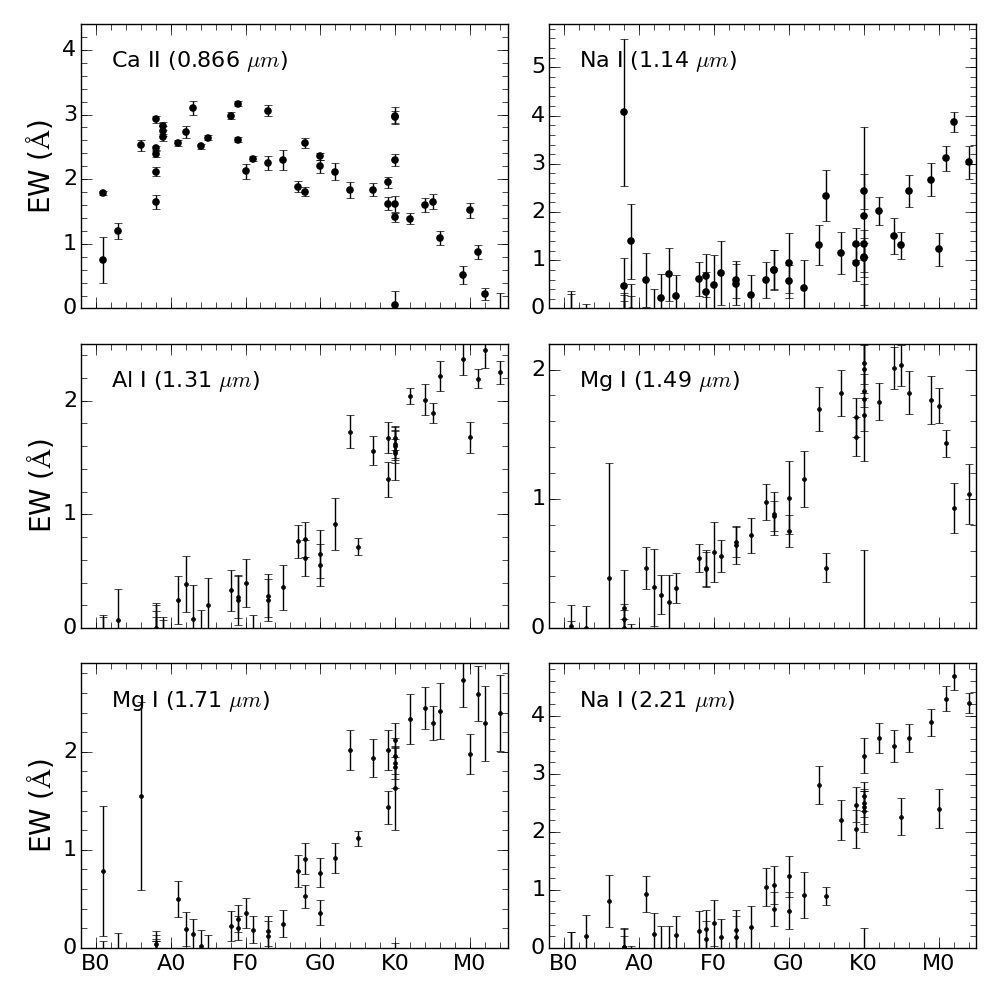
\includegraphics[height = 350px,width = 250px]{/Users/cmutnik/work/git/Spex-Young-Star-Atlas/figures/EW_SptType/obs/reproduce35_cutoff0_subplots_err}
\caption{ \protect{\bf Comparison of Spex \& uSpex} Shown here is a comparison of GSC 6801-186 using Spex before and after it was updated.}
\end{center}
\end{figure}


\begin{figure}[h!]
\begin{center}
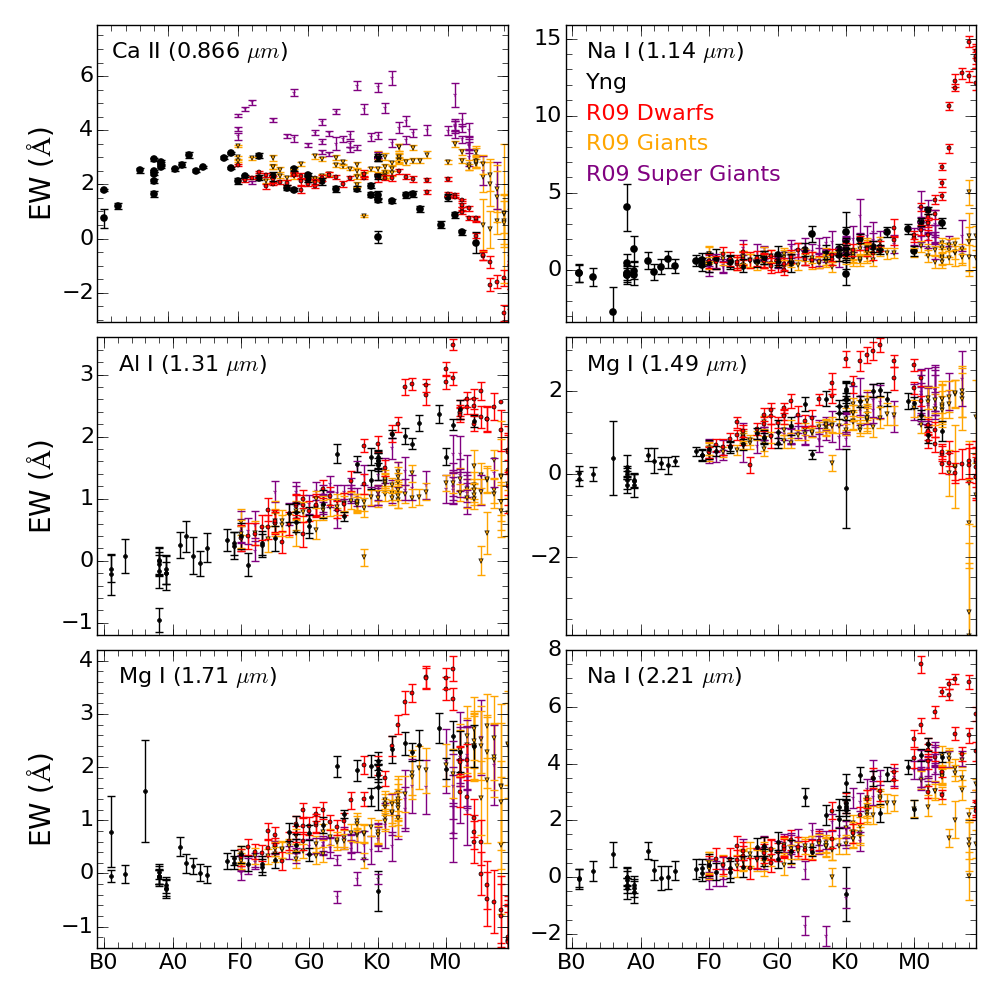
\includegraphics[height = 350px,width = 250px]{/Users/cmutnik/work/git/Spex-Young-Star-Atlas/figures/EW_SptType/obs_R09/EW_obs_calcR09_err.png}
\caption{ \protect{\bf Comparison of Spex \& uSpex} Shown here is a comparison of GSC 6801-186 using Spex before and after it was updated.}
\end{center}
\end{figure}

\begin{table}
\begin{center}
\caption{EW values for spectral features listed in Table~\ref{tab:features}.~\label{tab:EWvals}}
\begin{tabular}{l|c|c|c|c|c|c|c}
Object & Spectral Type & Ca II (0.866$\mu m$) & Na I (1.14 $\mu m$) & Al I (1.313 $\mu m$) & Mg I (1.485 $\mu m$) & Mg I (1.711$\mu m$) & Na I (2.206$\mu m$) \\
HD 146266 & A1V & 2.56299927871$\pm$0.0505902823735 & 0.593124316048$\pm$0.553721997646 & 0.247923195896$\pm$0.211153063071 & 0.467304907556$\pm$0.162599896949 & 0.498343619967$\pm$0.179011715613 & 0.928040199289$\pm$0.307913473327 \\
HD 143472 & A2V & 2.72620156086$\pm$0.0890465928405 & -0.124365182652$\pm$0.530925240599 & 0.391124557178$\pm$0.246336218988 & 0.317949507564$\pm$0.297752596569 & 0.191968496171$\pm$0.175898467241 & 0.248362913466$\pm$0.347114713752 \\
HD 145468 & A3V & 3.09676507059$\pm$0.105335208586 & 0.219012800854$\pm$0.493783546746 & 0.0822147058984$\pm$0.294680865998 & 0.260302944573$\pm$0.149758401131 & 0.140501549297$\pm$0.15304948548 & -0.0398126554199$\pm$0.411969668627 \\
HD 142424 & A4V & 2.50903380614$\pm$0.0418818508702 & 0.707624567334$\pm$0.546249292806 & -0.0422520066208$\pm$0.20311331033 & 0.203613953988$\pm$0.210989965198 & 0.0169708489128$\pm$0.166268738679 & -0.0105871358749$\pm$0.396645057413 \\
HD 142097 & A5V & 2.63724671857$\pm$0.0387032039504 & 0.249643364628$\pm$0.439152676298 & 0.206710796113$\pm$0.232352338186 & 0.313932023818$\pm$0.116300445526 & -0.0253045585246$\pm$0.156766454936 & 0.223030138592$\pm$0.332804727511 \\
HD 146899 & A8V & 2.98045841895$\pm$0.0563869594594 & 0.610106101858$\pm$0.357532070952 & 0.333645760799$\pm$0.179832027862 & 0.545505659787$\pm$0.108968849597 & 0.22816245596$\pm$0.153020819605 & 0.288821072073$\pm$0.355370706501 \\
HIP 73990 & A9V & 3.16901597018$\pm$0.0343419109672 & 0.332887913546$\pm$0.414429235798 & 0.244413455649$\pm$0.214388158541 & 0.455779985644$\pm$0.130985429993 & 0.204343512187$\pm$0.124168006378 & 0.152767555668$\pm$0.307654469178 \\
HD 147137 & A9V & 2.61193758312$\pm$0.0425581256529 & 0.674573918087$\pm$0.44666262191 & 0.278399220567$\pm$0.188724518059 & 0.462500930478$\pm$0.142401139772 & 0.298477576415$\pm$0.138773425249 & 0.321126397492$\pm$0.325174672103 \\
HIP 78933 & B1V & 1.79060453404$\pm$0.0292219340768 & -0.225324048904$\pm$0.524656105628 & -0.125192979484$\pm$0.223124527569 & -0.117885593152$\pm$0.176942022287 & -0.0473719265542$\pm$0.117590274704 & -0.0427072167468$\pm$0.31263596659 \\
HD 144470 & B1V & 0.748607183674$\pm$0.353534583215 & -0.189840080094$\pm$0.559123643051 & -0.216373644397$\pm$0.330432202688 & 0.0171548529069$\pm$0.165978517587 & 0.784746083483$\pm$0.6646177933 & -0.0827651446148$\pm$0.356267424344 \\
HD 138485 & B3V & 1.20021713217$\pm$0.123249228036 & -0.459617243235$\pm$0.558694012872 & 0.0728691201849$\pm$0.273736731925 & -0.000550825139467$\pm$0.174060490511 & -0.0173769510158$\pm$0.168111557896 & 0.204211970778$\pm$0.35979998636 \\
HD 147196 & B6/B7Vn & 2.52213176697$\pm$0.0903438021126 & -2.6952099117$\pm$1.56138778136 & 7.62443512689$\pm$3.1856674478 & 0.386186295866$\pm$0.88770200439 & 1.55196268513$\pm$0.956957467743 & 0.803768774883$\pm$0.444628821219 \\
HIP 70753 & B8V & 2.39216215594$\pm$0.0467874269198 & 0.458962358336$\pm$0.580555959477 & -0.0456916671113$\pm$0.194228420534 & -0.143675655878$\pm$0.218673469501 & -0.0615422387806$\pm$0.131477874233 & -0.114939972317$\pm$0.319223954394 \\
HIP 77909 & B8V & 2.48348877896$\pm$0.0356986682689 & -0.163081246205$\pm$0.492873464966 & -0.00935820466925$\pm$0.21377595358 & 0.00504509690005$\pm$0.132681167983 & -0.059001389929$\pm$0.133402159325 & 0.0181031682984$\pm$0.314243227268 \\
HIP 79031 & B8V & 2.92313532374$\pm$0.0490276065772 & -0.302182483479$\pm$0.453698453739 & 0.00544799276697$\pm$0.214957987998 & 0.0729167590449$\pm$0.116319630451 & 0.0364125924041$\pm$0.135172897128 & 0.0131169088652$\pm$0.323173228272 \\
HIP 78207 & B8V & 1.65203955311$\pm$0.108135748082 & 4.06821387941$\pm$1.52965998406 & -0.959455560465$\pm$0.193892811629 & 0.156428346797$\pm$0.291970334921 & -0.0501810116562$\pm$0.142423911101 & -0.295334129344$\pm$0.271627887931 \\
HD 144661 & B8V & 2.11294061833$\pm$0.0699405826986 & -0.30876422225$\pm$0.582168548989 & -0.169663219905$\pm$0.26599592733 & -0.266755666567$\pm$0.20203983247 & -0.0506584057615$\pm$0.182030672387 & -0.393030322988$\pm$0.365582143368 \\
HIP 76633 & B9V & 2.64639933676$\pm$0.0571975714836 & 1.38932051895$\pm$0.787411059967 & -0.197584323978$\pm$0.183866687156 & -0.278021156626$\pm$0.276539428908 & -0.269436993406$\pm$0.153867963159 & -0.268915126467$\pm$0.296323459459 \\
HIP 79599 & B9V & 2.81912816636$\pm$0.0655007572171 & -0.0537110373563$\pm$0.561134681749 & -0.135504189402$\pm$0.234606307094 & -0.175799896597$\pm$0.169716539558 & -0.221498328341$\pm$0.151378309157 & -0.401159910221$\pm$0.318235145645 \\
HD 143567 & B9V & 2.73921608292$\pm$0.0776068347864 & -0.346482479213$\pm$0.61236750112 & -0.195953579761$\pm$0.271542191608 & -0.142398928928$\pm$0.175474237143 & -0.285297003994$\pm$0.173195516811 & -0.531048709717$\pm$0.396335706349 \\
HD 137130 & F0V & 2.1187101502$\pm$0.109996007908 & 0.478070933429$\pm$0.623154941079 & 0.39646637362$\pm$0.212045327467 & 0.589204046313$\pm$0.231716916716 & 0.357126461238$\pm$0.151047460977 & 0.426814821898$\pm$0.390575353051 \\
HIP 79369 & F1V & 2.31937736651$\pm$0.0441335792305 & 0.736814084079$\pm$0.654702018937 & -0.0635755649691$\pm$0.181157059693 & 0.557835815852$\pm$0.121838301765 & 0.183160571817$\pm$0.137542232749 & 0.188382953399$\pm$0.307167404522 \\
HIP 82319 & F3V & 3.06056116029$\pm$0.0807534904999 & 0.596463524909$\pm$0.38397756934 & 0.249627706165$\pm$0.185266881861 & 0.667688662301$\pm$0.114577060666 & 0.170245506824$\pm$0.151203670633 & 0.305059034094$\pm$0.355544675942 \\
HD 146743 & F3V & 2.25045438173$\pm$0.103381509043 & 0.498907766341$\pm$0.425529772313 & 0.28519774038$\pm$0.188893372889 & 0.641715184661$\pm$0.14641976405 & 0.123924826338$\pm$0.147550400666 & 0.189563795999$\pm$0.358077586489 \\
HD 148153 & F5V & 2.29157107038$\pm$0.155742615121 & 0.269936653943$\pm$0.419986549644 & 0.360584111783$\pm$0.197482066422 & 0.718629501841$\pm$0.134359287276 & 0.249145967007$\pm$0.141302539988 & 0.364426688243$\pm$0.360840806691 \\
HIP 78977 & F7V & 1.88231995991$\pm$0.0851137562302 & 0.591071362265$\pm$0.376994867347 & 0.765500318479$\pm$0.145768284851 & 0.976080323192$\pm$0.139915093465 & 0.780749539409$\pm$0.163337054458 & 1.05022882044$\pm$0.325186301228 \\
HIP 71982 & F8V & 2.56060188894$\pm$0.0762131229772 & 0.798555225551$\pm$0.417017794526 & 0.620938065715$\pm$0.158607882372 & 0.868272743398$\pm$0.114204454237 & 0.526220430784$\pm$0.114845207605 & 0.673448419059$\pm$0.298182848716 \\
HD 142113 & F8V & 1.80715735375$\pm$0.065280032777 & 0.807408187185$\pm$0.411246825208 & 0.781155130065$\pm$0.151633735973 & 0.885590140425$\pm$0.168239206302 & 0.910486706422$\pm$0.161616718765 & 1.0795859872$\pm$0.324865620392 \\
HIP 61412 & G0V & 2.35262109221$\pm$0.0592524670013 & 0.563753159833$\pm$0.342778956876 & 0.555384500586$\pm$0.182710716484 & 0.752489322572$\pm$0.120869848394 & 0.357045604451$\pm$0.127130665563 & 0.644565751366$\pm$0.31402913356 \\
HD 148040 & G0V & 2.20053757099$\pm$0.101688995449 & 0.945525631363$\pm$0.625769325025 & 0.654320280283$\pm$0.208679881623 & 1.01022845396$\pm$0.282839563547 & 0.768391026907$\pm$0.144967719936 & 1.23273134043$\pm$0.352674224275 \\
HD 133748 & G2V & 2.11491753543$\pm$0.130076563777 & 0.434474969927$\pm$0.575014206003 & 0.916538128812$\pm$0.22486390158 & 1.153444896$\pm$0.218486634722 & 0.918078529889$\pm$0.151063331346 & 0.909761274454$\pm$0.399447968532 \\
GSC 06793-00994 & G4V & 1.82943169529$\pm$0.122746870859 & 1.30690699955$\pm$0.415157159775 & 1.72807407047$\pm$0.145474500598 & 1.69534120623$\pm$0.168896512136 & 2.01462884528$\pm$0.202897455379 & 2.80588135405$\pm$0.319450342068 \\
HBC 649 & G5V & -11.1492957606$\pm$0.138296074012 & 2.34180866524$\pm$0.527490396217 & 0.717166450005$\pm$0.0762831995013 & 0.468390267576$\pm$0.110335275431 & 1.11773082609$\pm$0.078148075599 & 0.891456500139$\pm$0.160107441526 \\
GSC 06801-00186 (oldSpx) & K0IV(e) & 1.61984274243$\pm$0.120570710423 & 1.0591344803$\pm$0.397727631834 & 1.60226758256$\pm$0.128100922757 & 2.05373888379$\pm$0.16316118595 & 1.95755982934$\pm$0.179357468494 & 2.3522143806$\pm$0.359138310598 \\
GSC 06801-00186 & K0IV(e) & 2.95767211472$\pm$0.089655798648 & 2.4310123804$\pm$0.358654746458 & 1.66734290193$\pm$0.0997144697786 & 2.00387638251$\pm$0.185044064236 & 2.11981869929$\pm$0.169535409392 & 2.49341840979$\pm$0.24360641565 \\
GSC 06793-01406 & G7V & 1.83580456818$\pm$0.0985098972086 & 1.15935055549$\pm$0.435042431319 & 1.56118822421$\pm$0.124230338098 & 1.82024696345$\pm$0.178207599741 & 1.93700364568$\pm$0.196430696348 & 2.19905355221$\pm$0.348279690303 \\
GSC 06213-00306AB & G9V & 1.62311949533$\pm$0.100699089538 & 1.33688888145$\pm$0.334508160925 & 1.67590599835$\pm$0.135603126358 & 1.63082307631$\pm$0.150460692068 & 2.01727644236$\pm$0.205822896899 & 2.46553921463$\pm$0.302468751134 \\
CD-25 11942 & K0V & 2.30203721938$\pm$0.0933113714974 & 1.05295210041$\pm$0.29715866087 & 1.61894223888$\pm$0.1227996101 & 1.83600132983$\pm$0.127216397988 & 1.88190541354$\pm$0.155949517283 & 2.41907848305$\pm$0.282451977842 \\
ScoPMS 214 & K0 / K2IV(e) & 1.40960995147$\pm$0.0646030261218 & 1.34696384811$\pm$0.285200757099 & 1.55725421307$\pm$0.1034028823 & 1.65167025243$\pm$0.12518212879 & 1.84319632851$\pm$0.207956359208 & 2.61279135438$\pm$0.250837860061 \\
HD 141813 & K0 / K1III+ & 0.0522366059582$\pm$0.215325641091 & 1.90968185145$\pm$1.84440442415 & -4.2141947175$\pm$1.91807297939 & -0.34729498768$\pm$0.954004026814 & -0.328293912507$\pm$0.377267225593 & -0.605255246685$\pm$0.942030372182 \\
HD 14311 & K0III & 2.98372410744$\pm$0.130486483868 & -0.235621959504$\pm$0.748171496459 & 1.5399700434$\pm$0.237686948718 & 1.77582395155$\pm$0.479009642276 & 1.62606181716$\pm$0.428611696093 & 3.31191465478$\pm$0.304486749895 \\
ScoPMS 44 & K2 / K2IV(e) & 1.3889969003$\pm$0.0833266847196 & 2.02571434786$\pm$0.290506093314 & 2.04011040489$\pm$0.0688496685997 & 1.75090733896$\pm$0.142686425786 & 2.33475689794$\pm$0.252900801427 & 3.61143957465$\pm$0.262246033924 \\
GSC 06793-00797 & K4V & 1.60031113319$\pm$0.109051356026 & 1.5075712139$\pm$0.373198133328 & 2.00969669174$\pm$0.134078990782 & 2.01372513049$\pm$0.162924086777 & 2.44607925918$\pm$0.210656806877 & 3.47565359877$\pm$0.279306273969 \\
ScoPMS 45 & K5V & 1.65273853222$\pm$0.112947580901 & 1.31570628777$\pm$0.280317733493 & 1.88916442278$\pm$0.0861445043609 & 2.03167702986$\pm$0.157571574221 & 2.28906517037$\pm$0.172955441274 & 2.26312018992$\pm$0.318849065173 \\
GSC 06208-00834 & K6V & 1.09074482544$\pm$0.114409678454 & 2.44347960709$\pm$0.329408071793 & 2.21599467146$\pm$0.13266864352 & 1.81975632486$\pm$0.167001528305 & 2.41397271201$\pm$0.286895531625 & 3.61671090122$\pm$0.247394413565 \\
Sco 160900.7-19085 & K9V & 0.514343006251$\pm$0.140045322506 & 2.66950891417$\pm$0.337549741634 & 2.36657195838$\pm$0.139699525493 & 1.76521322423$\pm$0.187559051826 & 2.7332592469$\pm$0.276913057035 & 3.88341235694$\pm$0.234850767647 \\
GSC 06213-00194 & M0V & 1.51725105738$\pm$0.116938423225 & 1.2256085875$\pm$0.34331501861 & 1.67751863431$\pm$0.137210739035 & 1.72162338964$\pm$0.137546498379 & 1.97365864576$\pm$0.203716608849 & 2.39838287043$\pm$0.333717952168 \\
RX J1602.0-2221 & M1V & 0.873189829957$\pm$0.104854326059 & 3.11276184212$\pm$0.266026953065 & 2.19429954266$\pm$0.0834867228653 & 1.43070263382$\pm$0.105364779771 & 2.59263526007$\pm$0.279087552975 & 4.29461948122$\pm$0.216707041632 \\
ScoPMS 008b & M2.5V & 0.224718222636$\pm$0.093494420688 & 3.86823577059$\pm$0.210885957247 & 2.44113951941$\pm$0.155155182822 & 0.929658191403$\pm$0.193929740494 & 2.28933326087$\pm$0.38516305596 & 4.67692259181$\pm$0.234564530035 \\
ScoPMS 46 & M4V & -0.152857282347$\pm$0.390248535915 & 3.03220912855$\pm$0.340121775754 & 2.2504680228$\pm$0.100939460749 & 1.03618751348$\pm$0.232044438502 & 2.39629039969$\pm$0.389163189136 & 4.22294456994$\pm$0.176365916766 \\
HIP 78721 & SC5.5-C71e & 1.8043779584$\pm$0.232999384521 & 1.64427489841$\pm$1.81687801297 & 0.361094770247$\pm$0.397536220191 & 1.0741530866$\pm$0.736641346734 & 0.325028958446$\pm$0.82252029215 & 3.72507899061$\pm$0.764627986149 \\
RX J1558.2-2328 & G9V & 1.95256353783$\pm$0.0830954335945 & 0.950527909068$\pm$0.373547463004 & 1.30773914642$\pm$0.151853067247 & 1.47955159358$\pm$0.150072345757 & 1.43237694534$\pm$0.167705730895 & 2.04366998376$\pm$0.323988650822 \\
\end{tabular}
\end{center}
\end{table}

\section{Comparison with Models}


  

  

\begin{figure}[h!]
\begin{center}
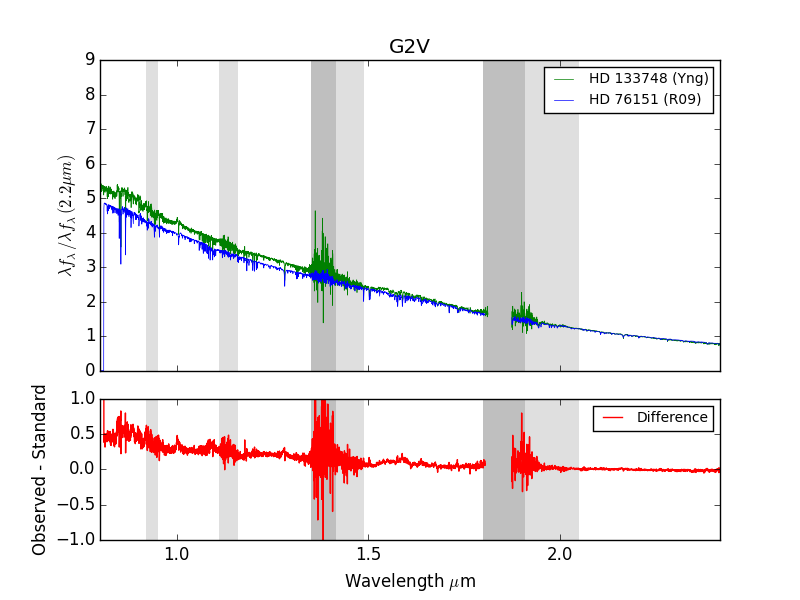
\includegraphics[height = 350px,width = 250px]{/Users/cmutnik/work/git/Spex-Young-Star-Atlas/figures/comparison/G2V/G2V_difference_observed_standard.png}
\caption{ \protect{\bf Comparison of Spex \& uSpex} Shown here is a comparison of GSC 6801-186 using Spex before and after it was updated.}
\end{center}
\end{figure}


\begin{figure}[h!]
\begin{center}
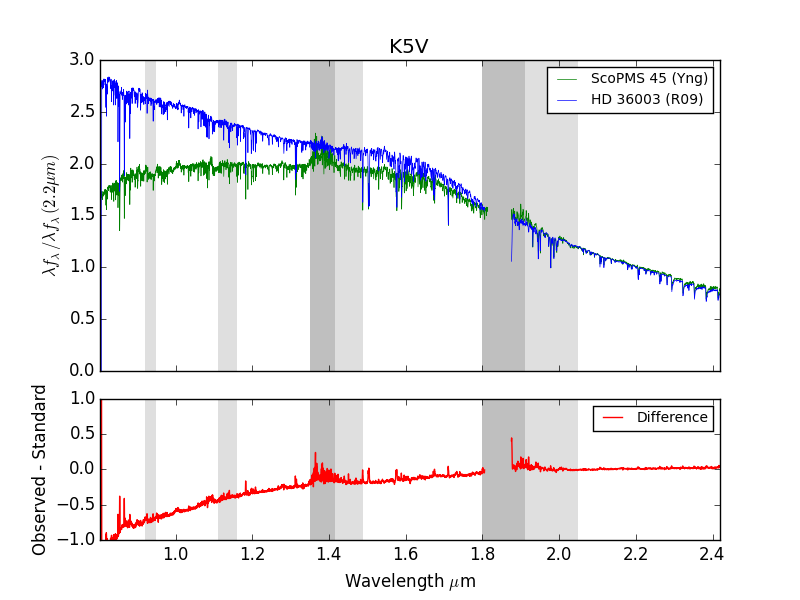
\includegraphics[height = 350px,width = 250px]{/Users/cmutnik/work/git/Spex-Young-Star-Atlas/figures/comparison/K5V/K5V.png}
\caption{ \protect{\bf Comparison of Spex \& uSpex} Shown here is a comparison of GSC 6801-186 using Spex before and after it was updated.}
\end{center}
\end{figure}

\section{Needed Citations}

\begin{bf}Sample Selection section\end{bf}
	\begin{itemize}
		\item{} NEED NAME OF PERSON WHO COMPLETE BINART SURVEY - DAVID L (GEMINI)?
		\item{} NEED NAME OF PERSON WHO COMPLETED ACCRETION DISK SURVEY
\end{itemize}

\begin{bf}Observation section\end{bf}
	\begin{itemize}
		%\item "Spextool: A Spectral Extraction Package for SpeX, a 0.8-5.5 Micron Cross Dispersed Spectrograph"\cite{Cushing_2004}
		\item{} \cite{Rayner_2003}
		\item{} cite whomever was referenced as identifying binaries \cite{Adam_Krauss_or_other_paper}
		\item{} cite whomever was referenced as identifying accretion disks \cite{Carpenter_2006}
		\item{} when upgrade of Spex occurred \cite{Spex}\\
		\item{} \cite{2mass_catalog_for_j_mags}
	\end{itemize} 


\begin{bf}Data Reduction and Analysis section\end{bf}
	\begin{itemize}
		\item{} Lord, S. D., 1992, NASA Technical Memorandum 103957
		\item{} Gemini Observatory for telluric transmission regions shown in gray on plots
  		\item{} Simbad
  
	\end{itemize}

\subsection{From Adam Kraus}
G, K, and early M stars: Kohler et al. (2000), Kraus et al. (2008), Lafreniere et al. (2014)

Mid/late M stars: Kraus et al. (2005), Bouy et al. (2006), Biller et al. (2011), Kraus $\&$ Hillenbrand (2012)

For disks, it's a little simpler. You can just use Carpenter et al. (2006, 2009) and Luhman $\&$ Mamajek (2012). 

\section{TEST}

is authorea updating?


\bibliography{/Users/cmutnik/work/git/Spex-Young-Star-Atlas/bibliography/biblio}{}

\end{document}
